\documentclass[10pt,xcolor=x11names,compress,aspectratio=169]{beamer}

%% =========================================================
%% Theme
%% =========================================================

\usetheme{Madrid}
\definecolor{mainblue}{RGB}{18,35,90}
\usecolortheme[named=mainblue]{structure}
\setbeamertemplate{footline}{%
  \begin{beamercolorbox}[wd=\paperwidth,ht=2.5ex,dp=1.5ex,center]{}%
    \usebeamerfont{footline}\color{mainblue}\insertframenumber
  \end{beamercolorbox}}
\setbeamertemplate{frametitle continuation}{}
\beamertemplatenavigationsymbolsempty
\setbeamerfont{title}{size=\Large}
\setbeamerfont{frametitle}{size=\large}
\setbeamertemplate{headline}{}
\setbeamertemplate{navigation symbols}{}

%% =========================================================
%% Packages
%% =========================================================

\usepackage{amsmath,amssymb,bm}
\usepackage{physics}
\usepackage{graphicx}
\usepackage{booktabs}
\usepackage{multirow}
\usepackage{tikz}
\usetikzlibrary{positioning,arrows.meta}
\usepackage{tcolorbox}
\tcbuselibrary{skins,breakable}
\usefonttheme{serif}

\graphicspath{{figures/}{./}}

%% =========================================================
%% Box Style
%% =========================================================

\tcbset{
  mybox/.style={
    enhanced, colback=white, colframe=mainblue,
    boxrule=0.6pt, arc=2pt,
    left=3pt, right=3pt, top=3pt, bottom=3pt
  }
}

%% =========================================================
%% Flowchart styles
%% =========================================================

\tikzset{
  fc/.style={draw=mainblue, rounded corners=2pt, fill=mainblue!6,
             align=center, text width=5.3cm, font=\scriptsize,
             inner sep=2.5pt, minimum height=0.5cm},
  fcd/.style={fc, fill=mainblue!18},
  fa/.style={-{Stealth[length=1.6mm]}, mainblue, thick}
}

%% =========================================================
%% Metadata
%% =========================================================

\title{%
  \parbox{0.78\linewidth}{\centering
    Rydberg Atomic Receivers\\
    for Future Wireless Communications}}
\author{P SRIHARI\\25SP06015}
\institute{M.Tech \\ Signal Processing \& Communications\\
  Indian Institute of Technology Bhubaneswar}

%% =========================================================
\begin{document}
%% =========================================================

%% ---- 1. Title (unchanged) --------------------------------
\begin{frame}[plain]
\begin{tikzpicture}[remember picture, overlay]

  \draw[mainblue, line width=1.2pt]
    ([yshift=-1.55cm]current page.north west) --
    ([yshift=-1.55cm]current page.north east);

  \node[anchor=north west, inner sep=0pt, text width=7cm, align=left]
    at ([xshift=12pt, yshift=-8pt]current page.north west)
    {\color{mainblue}\scriptsize
      \textbf{Indian Institute of Technology Bhubaneswar}\\[1pt]
      \textit{School of Electrical and Computer Science}};

  \node[anchor=north east, inner sep=0pt]
    at ([xshift=-10pt, yshift=-4pt]current page.north east)
    {\includegraphics[height=1.45cm]{IITBBS_Logo.png}};

  \node[anchor=center]
    at (current page.center)
    {\parbox{0.80\linewidth}{\centering
      {\color{mainblue}\LARGE\textbf{Rydberg Atomic Receivers\\[4pt]
      for Future Wireless Communications}}\\[10pt]
      {\normalsize\textbf{P SRIHARI}}\\[2pt]
      {\small 25SP06015}\\[2pt]
      {\small M.Tech in Signal Processing \& Communications}
    }};

  \node[anchor=south, inner sep=10pt]
    at ([yshift=30pt]current page.south)
    {\parbox{0.85\linewidth}{\centering\small
      \textit{Under the Supervision of :}\ Dr.\ Bharatram Ramkumar,\ \textit{Associate Professor}\\[3pt]
      \textit{Co-Supervisior :}\ Dr.\ Soumya Prakash Dash,\ \textit{Associate Professor}
    }};
\end{tikzpicture}
\end{frame}

%% ---- 2. Outline ------------------------------------------
\begin{frame}{Outline}
\begin{columns}[T]
\column{0.55\textwidth}
\begin{enumerate}\setlength\itemsep{6pt}
  \item Introduction and literature survey
  \item \textbf{Part A:} Harnessing Rydberg atomic receivers~\cite{chen2025harnessing}
  \begin{itemize}\small
    \item Four-level model, EIT/AT spectrum, distortion
    \item LO-dressed receiver, SNR versus distance
  \end{itemize}
  \item \textbf{Part B:} Channel estimation for Rydberg atomic receivers~\cite{xu2025channel}
  \begin{itemize}\small
    \item Atomic MIMO model, GD / PGD / biased GS, CRLB
    \item 1D and 2D array results
  \end{itemize}
  \item Research gaps and future work
\end{enumerate}
\column{0.40\textwidth}
\begin{tcolorbox}[mybox]
  \small\textbf{Work done so far}
  \begin{itemize}\footnotesize\setlength\itemsep{2pt}
    \item Literature survey on Rydberg atomic receivers
    \item Four-level Lindblad model in QuTiP: Figs.~3--6 of~\cite{chen2025harnessing}
    \item GD, PGD, biased GS and CRLB in MATLAB: Figs.~3--5 of~\cite{xu2025channel}
    \item Limitations and research gaps identified
  \end{itemize}
\end{tcolorbox}
\end{columns}
\end{frame}

%% ---- 3. Motivation ---------------------------------------
\begin{frame}{Rydberg Atomic Receivers: Motivation}
\begin{center}
  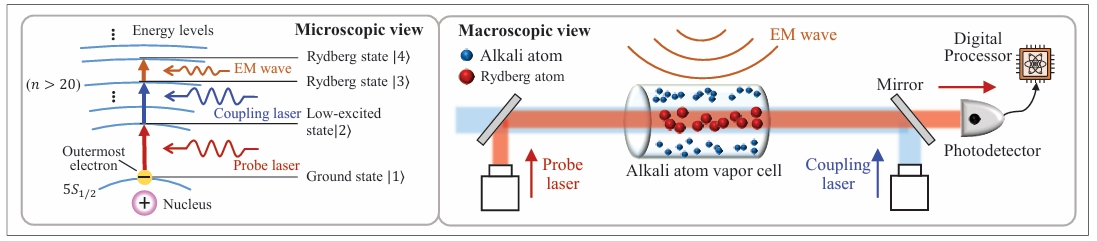
\includegraphics[width=0.92\textwidth]{rare_setup.png}\\[-1pt]
  {\tiny Microscopic (four-level excitation) and macroscopic (vapour cell) view. Adapted from~\cite{cui2026rare}.}
\end{center}
\vspace{-1mm}
\begin{columns}[T]
\column{0.48\textwidth}
\begin{tcolorbox}[mybox]
  \small\textbf{Properties of conventional receivers}
  \begin{itemize}\footnotesize\setlength\itemsep{1pt}
    \item Antenna size $\approx\lambda/2$ ($>50$~cm below 100~MHz)
    \item Front-end thermal noise ($-174$~dBm/Hz)
    \item One resonant antenna and RF chain per band
    \item Weak-field sensitivity limited by the antenna aperture and receiver noise
  \end{itemize}
\end{tcolorbox}
\column{0.48\textwidth}
\begin{tcolorbox}[mybox]
  \small\textbf{Properties of Rydberg atomic receivers}
  \begin{itemize}\footnotesize\setlength\itemsep{1pt}
    \item Rydberg atoms ($n>20$): size $\propto n^2$, very large dipole moment
    \item Probe $|1\rangle\!\to\!|2\rangle$, coupling $|2\rangle\!\to\!|3\rangle$, RF $|3\rangle\!\leftrightarrow\!|4\rangle$
    \item RF field read optically from probe transmission (EIT/AT)
    \item $\sim$1~cm cell for any carrier; band set by the choice of Rydberg levels
  \end{itemize}
\end{tcolorbox}
\end{columns}
\end{frame}

%% ---- 4. Literature survey --------------------------------
\begin{frame}{Literature Survey}
\small
\renewcommand{\arraystretch}{1.3}
\begin{tabular}{p{3.2cm}p{3.4cm}p{7.4cm}}
\toprule
\textbf{Work} & \textbf{Focus} & \textbf{Key contribution}\\
\midrule
Cui \textit{et al.}, 2024 (arXiv)~\cite{cui2026rare} & Overview of RAREs & Architecture, sensitivity and bandwidth; multi-band reception; open problems incl.\ channel estimation\\
Chen \textit{et al.}, 2025~\cite{chen2025harnessing} & LO-free and LO-dressed receivers & SNR, MI, SER and distortion regions from the Lindblad model (QuTiP)\\
Cui \textit{et al.}, 2025 (JSAC)~\cite{cui2025towards} & Atomic MIMO & Biased phase-retrieval model; biased GS and EM-GS detectors; CRLB\\
Xu \textit{et al.}, 2025~\cite{xu2025channel} & Channel estimation & Taylor linearisation; GD (1D), PGD with rank-$L_k$ SVD (2D); CRLB\\\bottomrule
\end{tabular}
\vspace{3mm}
\begin{itemize}\footnotesize
  \item Two modelling approaches exist: the \textbf{LO-dressed mixer} model~\cite{chen2025harnessing}
  and the \textbf{magnitude-only phase-retrieval} model~\cite{cui2025towards,xu2025channel}
\end{itemize}
\end{frame}

%% =========================================================
%% PART A: Chen et al.
%% =========================================================

%% ---- 5. Four-level model + setup -------------------------
\begin{frame}{Part A~\cite{chen2025harnessing}: Four-Level Model and Simulation Setup}
\begin{columns}[T]
\column{0.55\textwidth}
\footnotesize
\setlength{\abovedisplayskip}{3pt}\setlength{\belowdisplayskip}{3pt}
\setlength{\abovedisplayshortskip}{3pt}\setlength{\belowdisplayshortskip}{3pt}
\textcolor{mainblue}{\textbf{Energy levels (Cs)}}\\[1pt]
$|1\rangle{=}6S_{1/2}\to|2\rangle{=}6P_{3/2}\to|3\rangle{=}47D_{5/2}\to|4\rangle{=}48P_{3/2}$;
probe $\Omega_p$, coupling $\Omega_c$, RF $\Omega$

\vspace{3mm}
\textcolor{mainblue}{\textbf{Hamiltonian (rotating frame)}}
{\setlength{\arraycolsep}{3pt}
\[
  \mathbf H=\frac{\hbar}{2}
  \begin{bmatrix}
  0 & \Omega_p & 0 & 0\\
  \Omega_p & -2\Delta_p & \Omega_c & 0\\
  0 & \Omega_c & -2(\Delta_p{+}\Delta_c) & \Omega\\
  0 & 0 & \Omega & -2(\Delta_p{+}\Delta_c{+}\Delta_{RF})
  \end{bmatrix}
\]}

\vspace{1mm}
\textcolor{mainblue}{\textbf{Lindblad master equation}} (steady state solved in QuTiP~5.3~\cite{johansson2012qutip})
\[
  \dot{\bm\rho}=-\tfrac{j}{\hbar}[\mathbf H,\bm\rho]+\mathcal L(\bm\rho)=0
\]

\vspace{1mm}
\textcolor{mainblue}{\textbf{Probe power at the photodetector}}
\[
  P_{out}=P_{in}\,e^{-k_pL\,\mathrm{Im}(\chi)}
\]
\[
  \chi=C_0\rho_{21},\qquad C_0=-\frac{2N_0\wp_{12}}{\epsilon_0\hbar\Omega_p}
\]
{\scriptsize $k_p=2\pi/\lambda_p$, $L$: cell length, $N_0$: atom density}

\column{0.42\textwidth}
\vspace{4mm}
\footnotesize
\renewcommand{\arraystretch}{1.25}
\begin{tabular}{ll}
\toprule
\textbf{Parameter} & \textbf{Value}\\
\midrule
$L$, $N_0$ & 1~cm, $10^{15}$~m$^{-3}$\\
$\Omega_p/2\pi$, $\Omega_c/2\pi$ & 8~MHz, 1~MHz\\
$\gamma_2,\gamma_3,\gamma_4$ ($/2\pi$) & 5.2~MHz, 3.9~kHz, 1.7~kHz\\
$\lambda_p$, beam diam. & 852~nm, 0.76~mm\\
$P_{in}$ & 39.08~$\mu$W\\
$\Omega_{LO}/2\pi$, $\Delta f$ & 4.23~MHz, 150~kHz\\
$f_{RF}$, $B$ & 3.5~GHz, 1~MHz\\
$G_{Tx}=G_{Rx}$, $G_{LNA}$ & 2.15~dBi, 20~dB\\
$R_L$, $D$, $\eta_{\rm eff}$ & 50~$\Omega$, 0.55~A/W, 0.8\\
$\sigma_{BGN}$, $T$ & $-90$~dBm, 290~K\\
$\tilde\epsilon$ & 0.5\%\\
\bottomrule
\end{tabular}\\[3pt]
{\tiny Parameters from Sections IV--V of~\cite{chen2025harnessing}.}
\end{columns}
\end{frame}

%% ---- 6. EIT/AT surface -----------------------------------
\begin{frame}{Part A~\cite{chen2025harnessing}: EIT/AT Response of the LO-free Receiver}
\begin{columns}[T]
\column{0.55\textwidth}
\begin{center}
  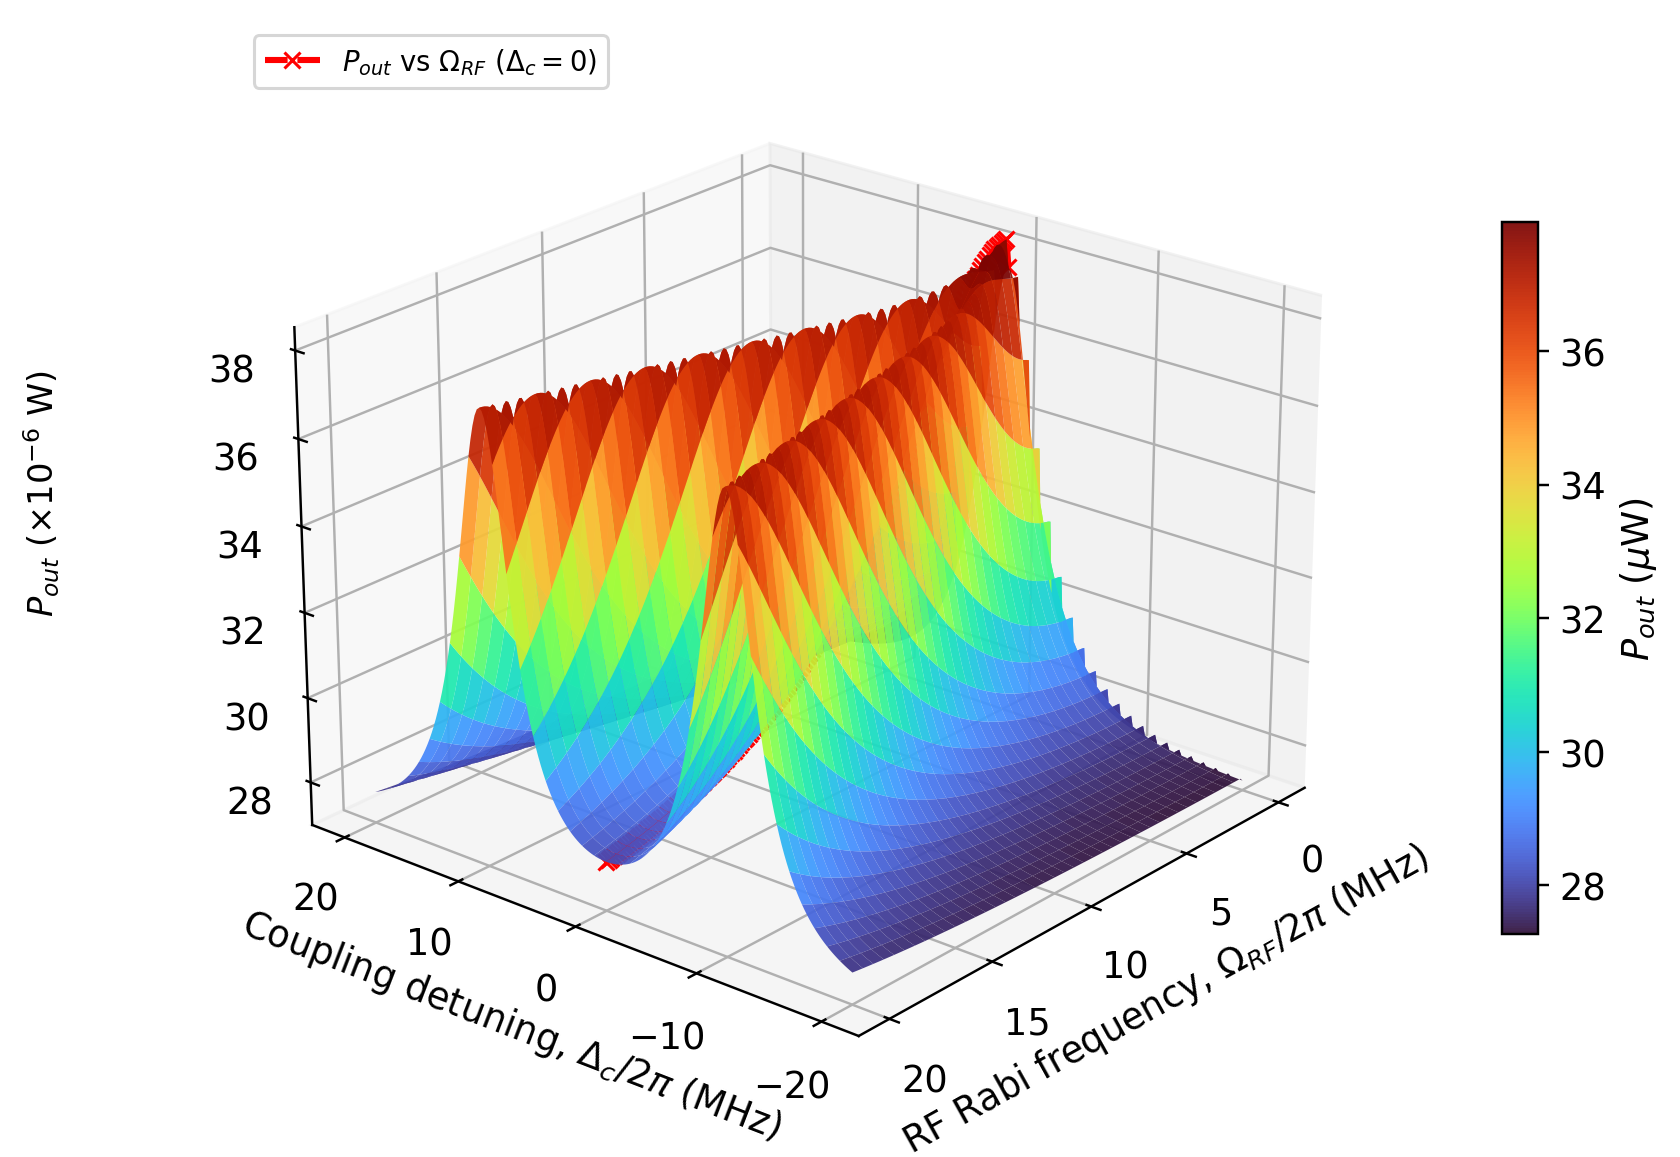
\includegraphics[width=\linewidth,height=0.72\textheight,keepaspectratio]{h_fig3_surface.png}\\
  {\tiny $P_{out}$ versus $\Delta_c$ and $\Omega_{RF}$ (Fig.~3 of~\cite{chen2025harnessing})}
\end{center}
\column{0.42\textwidth}
\footnotesize
\textbf{Graph generation}
\begin{itemize}\setlength\itemsep{1pt}
  \item Grid of $(\Delta_c,\Omega_{RF})$; at each point build $\mathbf H$
  \item QuTiP steady state $\to\rho_{21}\to\chi\to P_{out}$
  \item $P_{out}=P_{in}\,e^{-k_pL\,\mathrm{Im}(\chi)}$, with $\chi=C_0\rho_{21}$
\end{itemize}
\vspace{2mm}
\textbf{Observations}
\begin{itemize}\setlength\itemsep{2pt}
  \item $\Omega_{RF}=0$: coupling laser opens a transparency window (EIT) at $\Delta_c=0$
  \item RF field couples $|3\rangle\leftrightarrow|4\rangle$ and splits the peak into two AT peaks separated by $\Omega_{RF}$
  \item Red line: transmission at $\Delta_c=0$ falls as $\Omega_{RF}$ grows
  \item Peak $P_{out}=38.3~\mu$W from $P_{in}=39.08~\mu$W; $P_{in}$ only scales the curve
\end{itemize}
\end{columns}
\end{frame}

%% ---- 7. Slices + distortion ------------------------------
\begin{frame}{Part A~\cite{chen2025harnessing}: EIT/AT Spectra and Distortion Region}
\begin{columns}[T]
\column{0.53\textwidth}
\begin{center}
  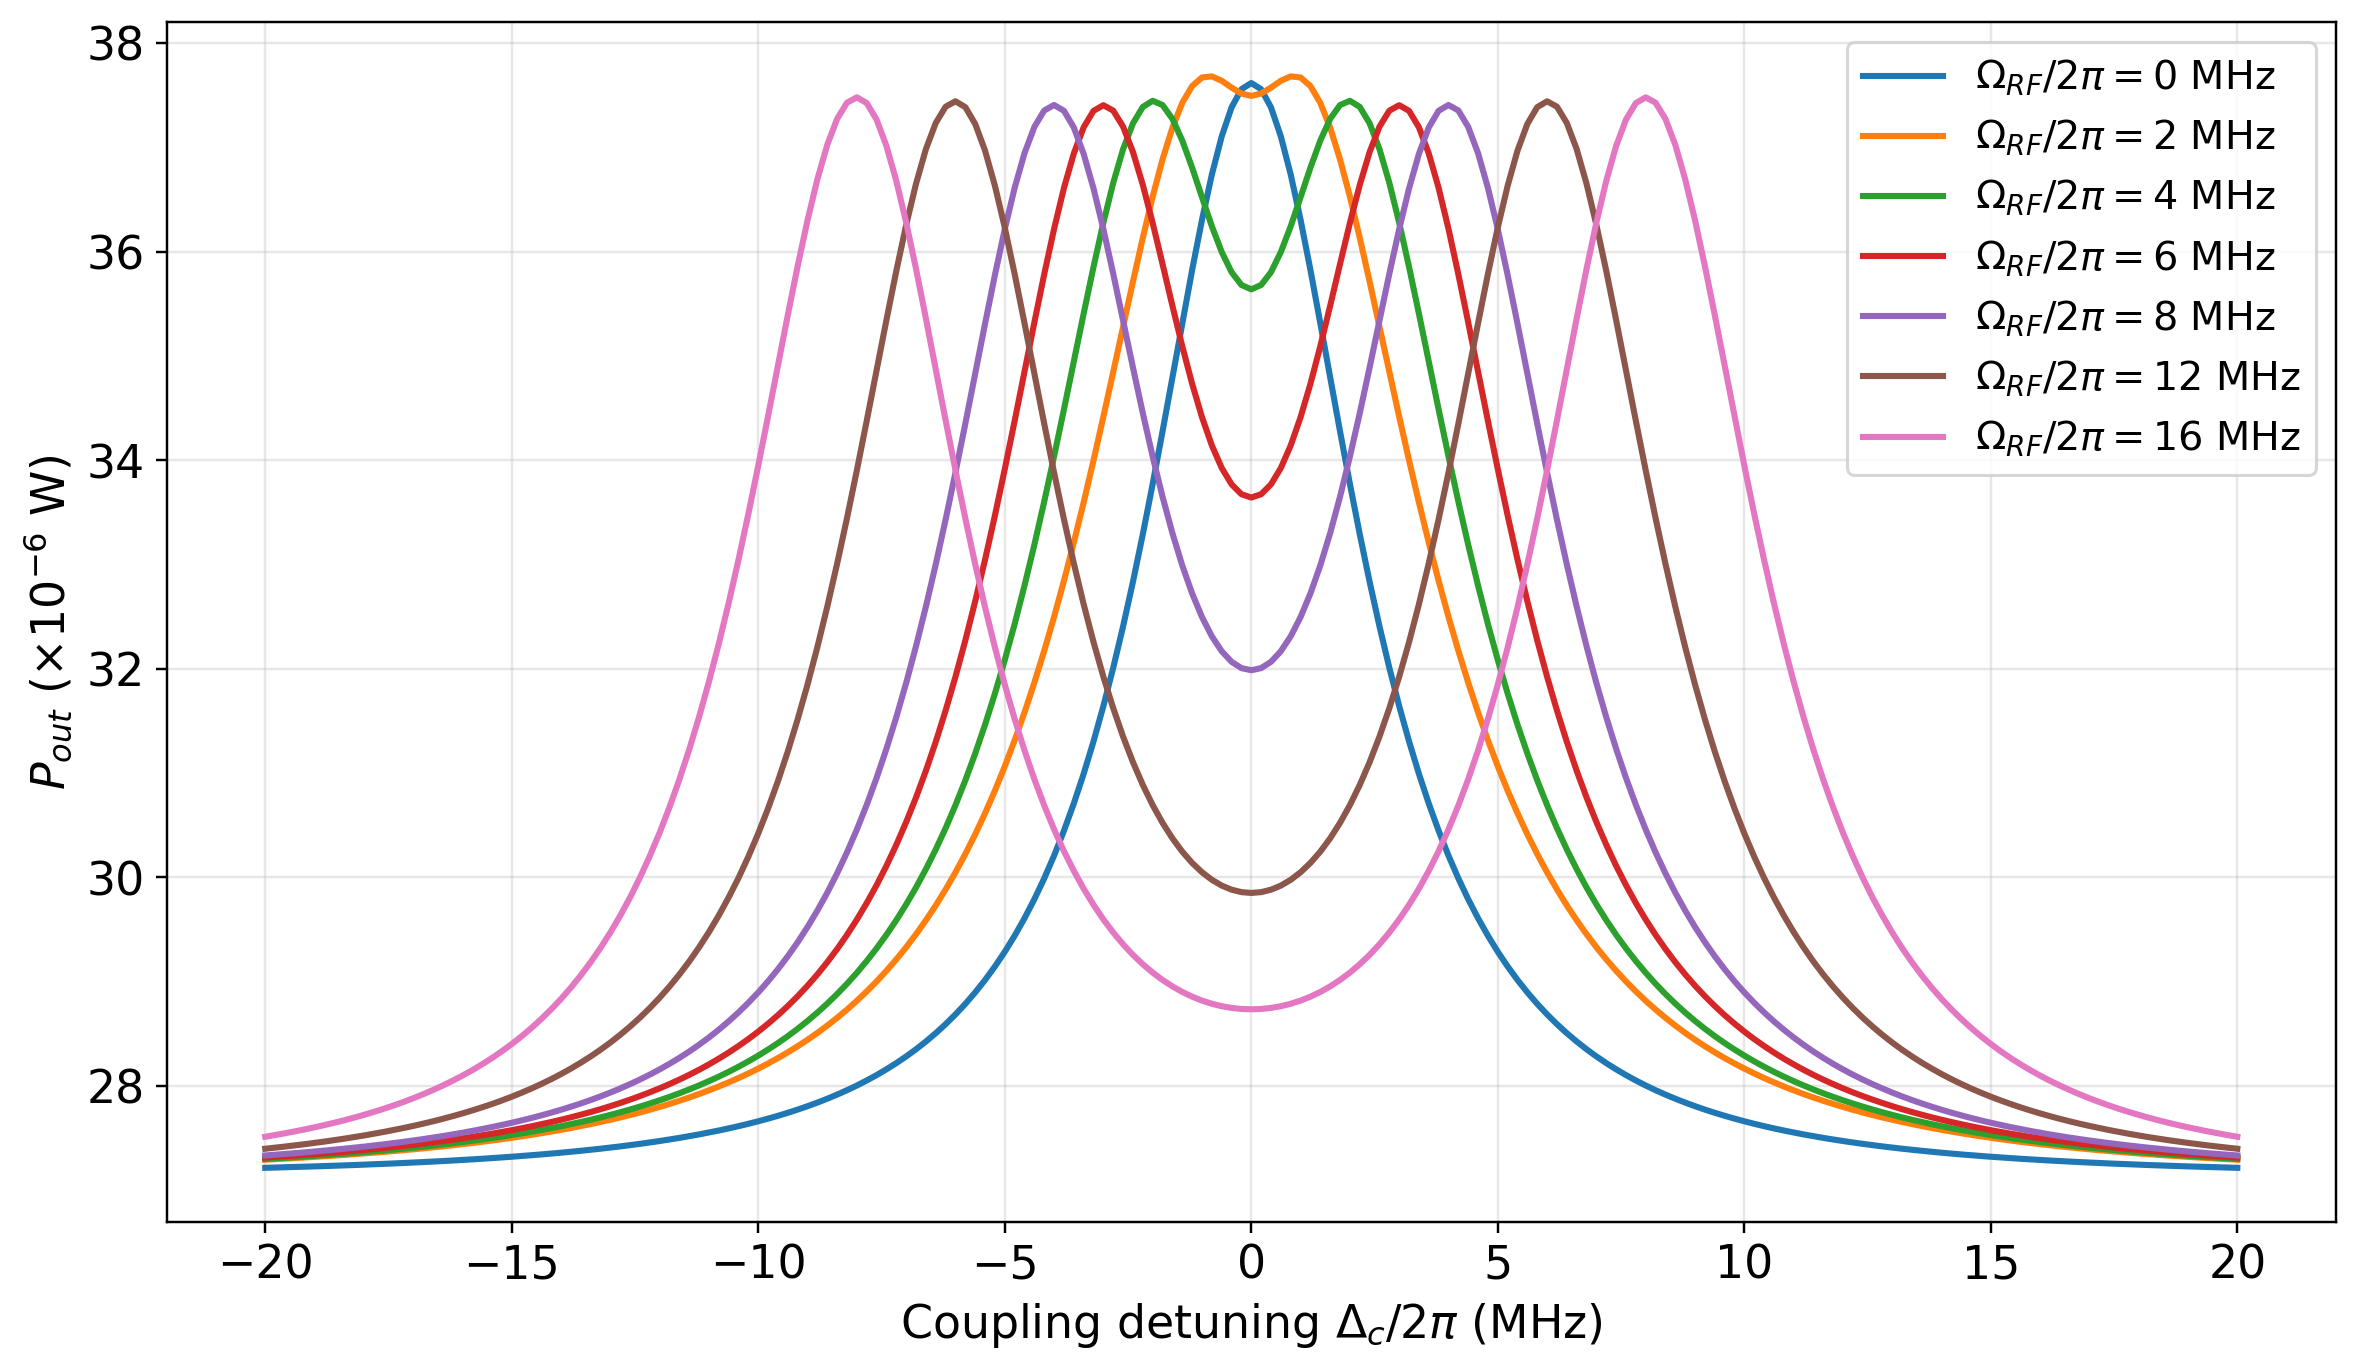
\includegraphics[width=\linewidth,height=0.46\textheight,keepaspectratio]{h_fig3_slices.png}\\
  {\tiny Spectra at fixed $\Omega_{RF}$ (rows of the surface)}
\end{center}
\column{0.44\textwidth}
\begin{center}
  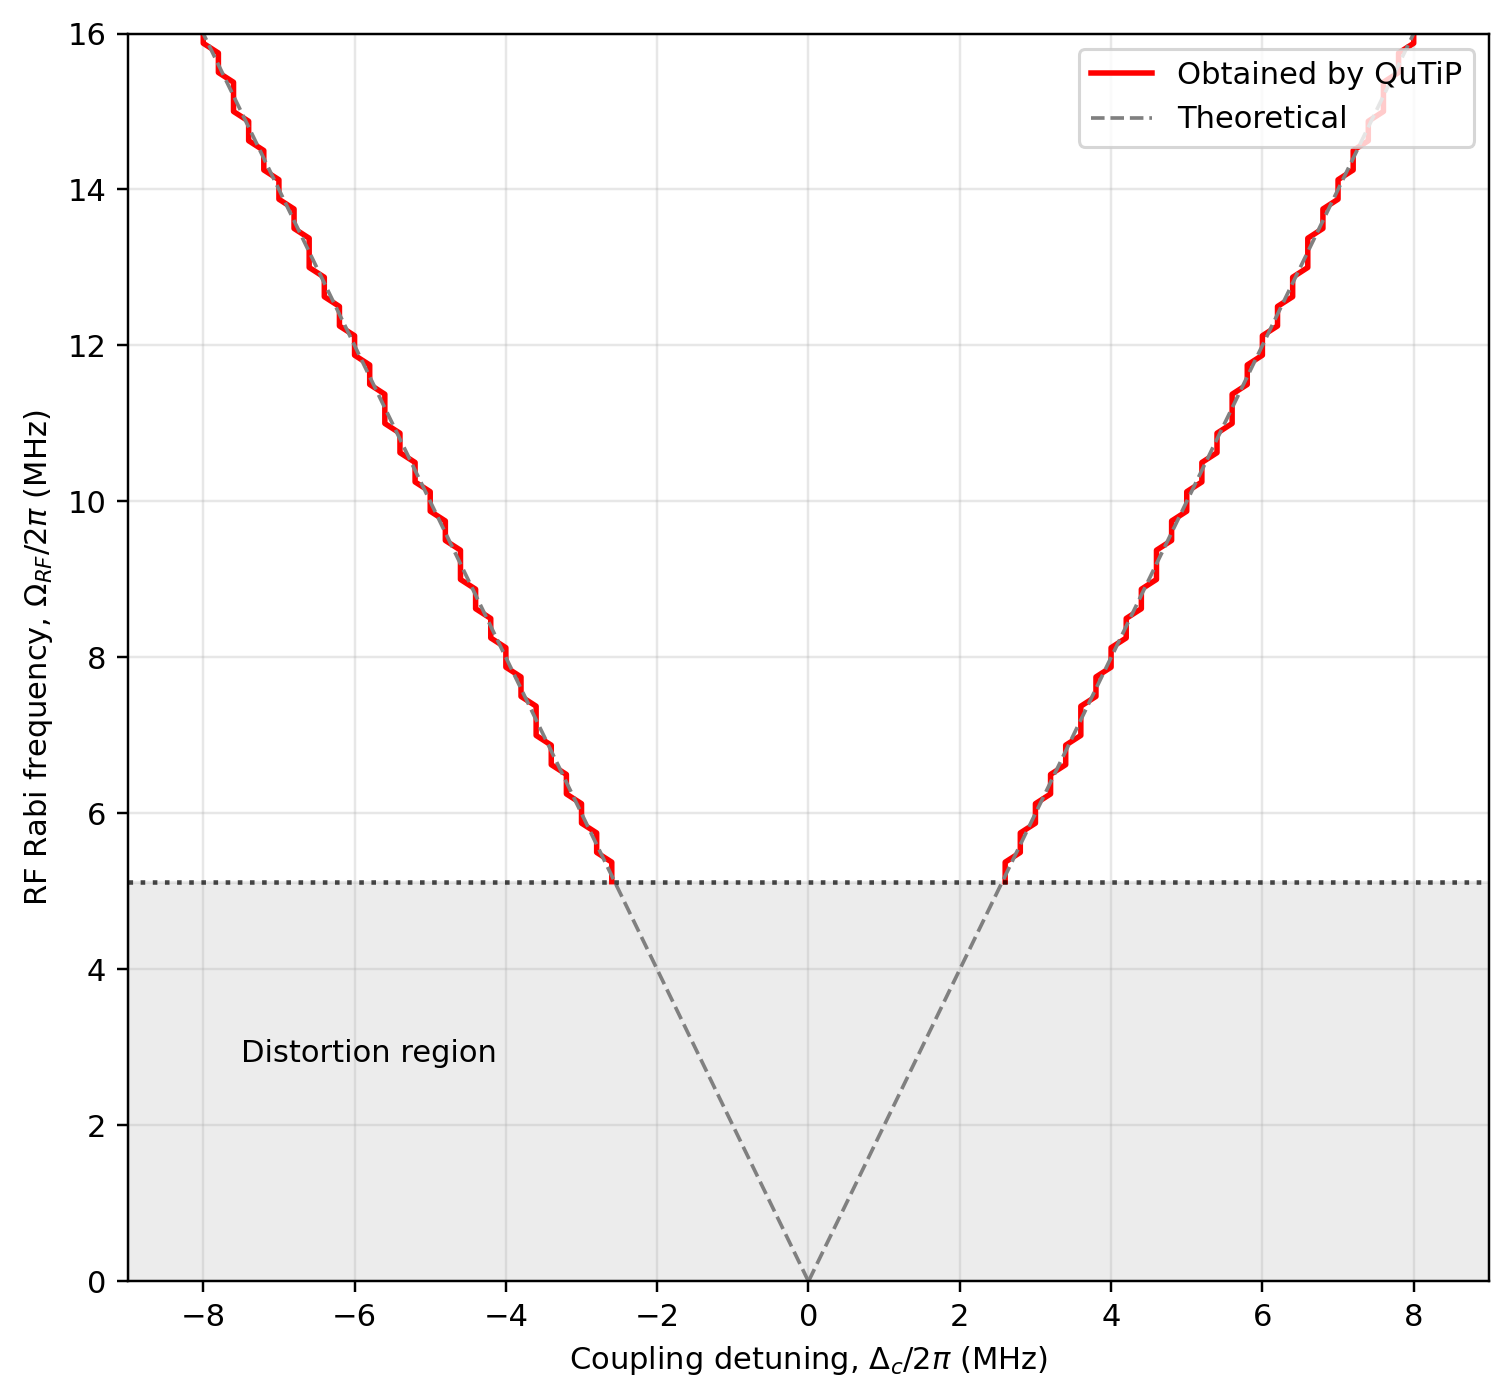
\includegraphics[width=\linewidth,height=0.46\textheight,keepaspectratio]{h_fig4_distortion.png}\\
  {\tiny AT peak positions and distortion region (Fig.~4 of~\cite{chen2025harnessing})}
\end{center}
\end{columns}
\vspace{1mm}
\footnotesize
\begin{itemize}\setlength\itemsep{2pt}
  \item \textbf{Graph generation:} surface data (no new solution) $\to$ two AT peaks in each row $\to$ peak
        separation $\to$ compare with EIT linewidth (FWHM $5.19$~MHz) $\to$ threshold $\Omega_{RF,th}$
  \item Above the threshold the peaks follow $\Delta_c=\pm\Omega_{RF}/2$
  \item Below $\Omega_{RF}/2\pi=5.125$~MHz the peaks merge and $\Omega_{RF}$ cannot be read: distortion region (paper $\approx5.5$~MHz)
\end{itemize}
\end{frame}

%% ---- 8. LO-dressed ---------------------------------------
\begin{frame}{Part A~\cite{chen2025harnessing}: LO-dressed Receiver and Linear Dynamic Range}
\begin{columns}[T]
\column{0.52\textwidth}
\begin{center}
  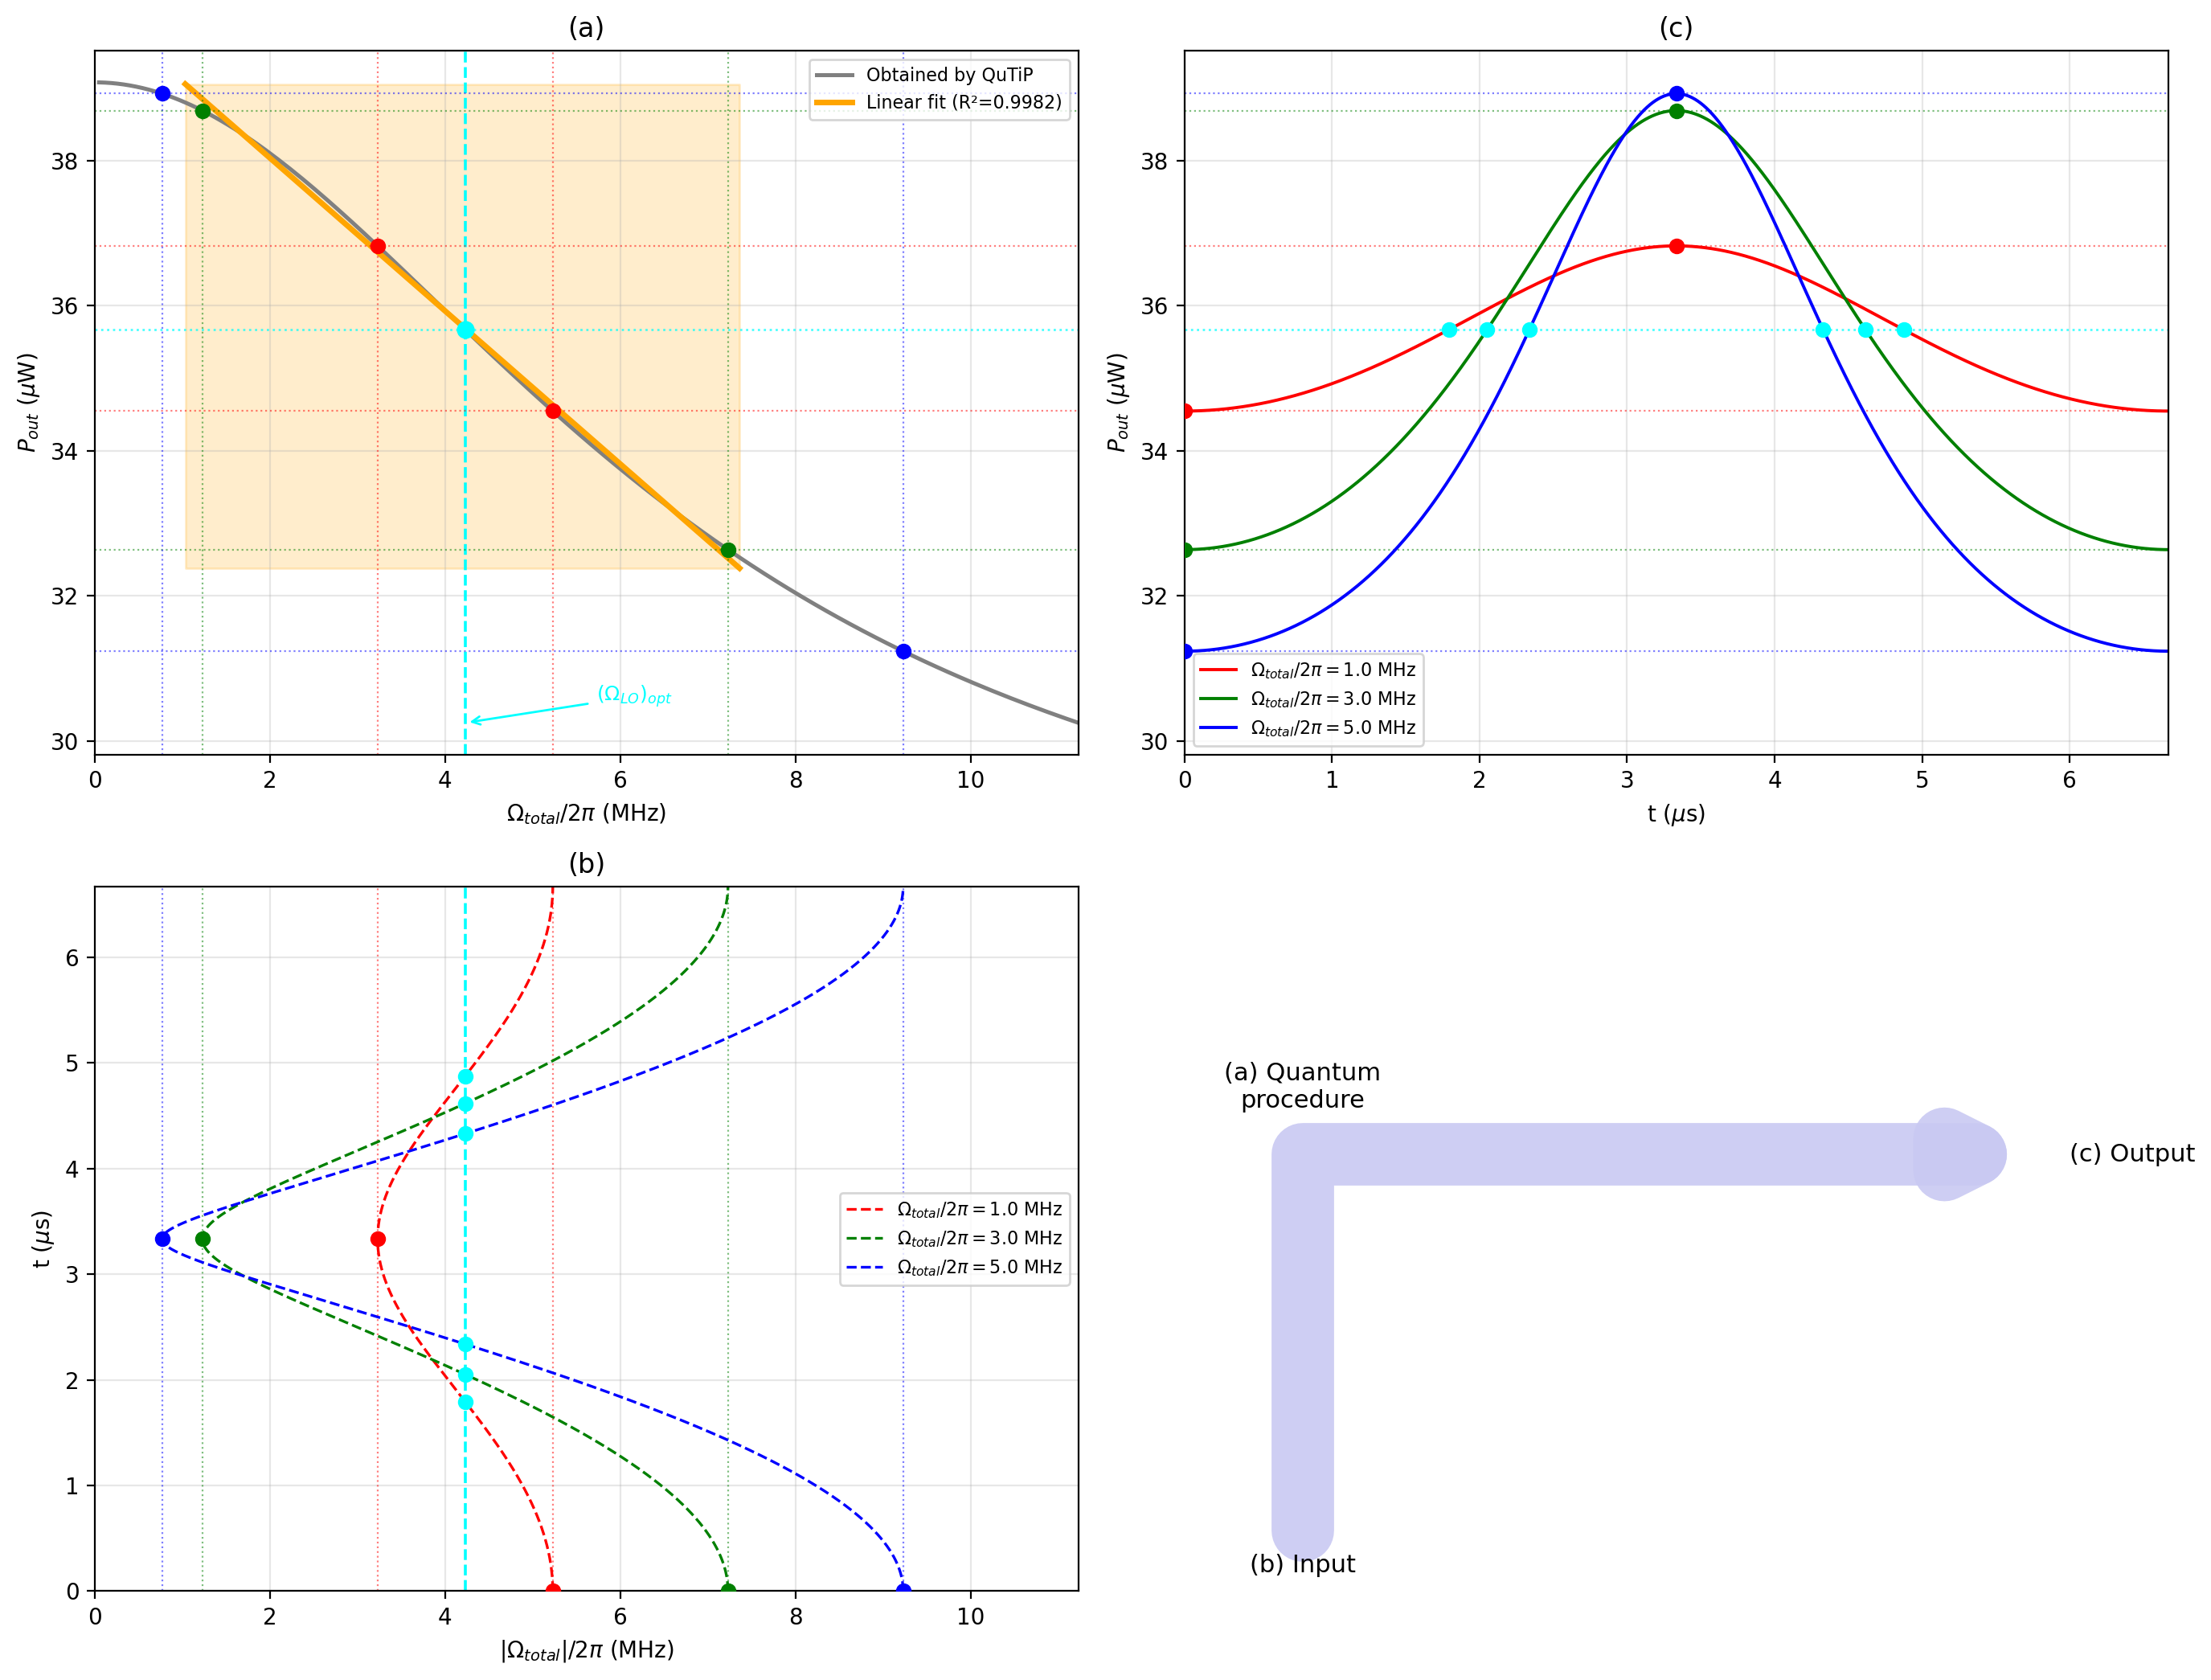
\includegraphics[width=\linewidth,height=0.72\textheight,keepaspectratio]{h_fig5_lodressed.png}\\
  {\tiny (a) $P_{out}$ vs $\Omega_{total}$, (b) input, (c) output (Fig.~5 of~\cite{chen2025harnessing})}
\end{center}
\column{0.45\textwidth}
\footnotesize
\textbf{Model} (atoms act as a mixer, $\Omega_{RF}\ll\Omega_{LO}$)
\[
  \Omega_{total}(t)=\big|\Omega_{LO}+e^{j(2\pi\Delta f t+\Delta\phi)}\Omega_{RF}\big|
\]
\[
  P_{out}(t)\approx\bar P_0+\kappa\,\Omega_{RF}\cos(2\pi\Delta f t+\Delta\phi)
\]
\textbf{Graph generation}
\begin{itemize}\setlength\itemsep{1pt}
  \item (a) $\Omega_{total}$ grid $\to$ QuTiP ($\gamma_3{=}\gamma_4{=}0$) $\to P_{out}(\Omega_{total})$ $\to$ linear fit ($R^2\geq0.998$) $\to\kappa$
  \item (b) $\Omega_{RF},\Delta f\to\Omega_{total}(t)$
  \item (c) $\Omega_{total}(t)\to$ curve (a) $\to P_{out}(t)$
\end{itemize}
\vspace{1mm}
\textbf{Observations}
\begin{itemize}\setlength\itemsep{1pt}
  \item Linear range $[1.03,7.36]$~MHz (paper $\approx[1.3,7.2]$)
  \item $\Omega_{RF}=1,3$~MHz: sinusoidal output; $5$~MHz: distorted
\end{itemize}
\end{columns}
\end{frame}

%% ---- 9. SNR models ---------------------------------------
\begin{frame}{Part A~\cite{chen2025harnessing}: SNR Models of the LO-free and LO-dressed Receivers}
\begin{columns}[T]
\column{0.48\textwidth}
\footnotesize
\setlength{\abovedisplayskip}{3pt}\setlength{\belowdisplayskip}{3pt}
\textcolor{mainblue}{\textbf{Link budget (both receivers)}}
\[
  P_{Rx}=|E_{RF}|^2=\frac{P_{Tx}G_{Tx}\eta_0}{4\pi d^2},\qquad
  \Omega_{RF}=\frac{|E_{RF}|\,\wp_{RF}}{\hbar}
\]
\vspace{1mm}
\textcolor{mainblue}{\textbf{LO-free receiver}}
\begin{itemize}\setlength\itemsep{1pt}
  \item Observation: $z=\frac{\hbar}{\wp_{RF}}\Omega_{RF}=\big|\sqrt{P_{Rx}}\,hx+n_{Ry}\big|$ (magnitude only)
  \item Noise: background $\sigma^2_{BGN}$, quantum projection $\sigma^2_{QPN}$, observation uncertainty $\sigma^2_{UN}=(\tilde\epsilon E_{RF})^2$
\end{itemize}
\[
  \mathrm{SNR}_{Ry}=\frac{P_{Rx}|h|^2}{\sigma^2_{BGN}+\sigma^2_{QPN}+\tilde\epsilon^2P_{Rx}}
\]
\begin{itemize}\setlength\itemsep{1pt}
  \item Noise grows with the signal: as $P_{Rx}\to\infty$, $\mathrm{SNR}_{Ry}\to1/\tilde\epsilon^2=46.02$~dB ($\tilde\epsilon=0.5\%$)
\end{itemize}
\column{0.49\textwidth}
\footnotesize
\setlength{\abovedisplayskip}{3pt}\setlength{\belowdisplayskip}{3pt}
\textcolor{mainblue}{\textbf{LO-dressed receiver}}
\begin{itemize}\setlength\itemsep{1pt}
  \item Photocurrent at $\Delta f$: $I_{AC}=D|\kappa|\Omega_{RF}$; after load $R_L$ and LNA gain $G_{LNA}$:
\end{itemize}
\[
  \mathrm{SNR}_{Ry,LO}=
  \frac{G_{LNA}R_LD^2\kappa^2\big(\wp_{RF}/\hbar\big)^2P_{Rx}|h|^2}
       {G_{LNA}R_LD^2\big[\kappa^2\big(\wp_{RF}/\hbar\big)^2\sigma^2_{BGN}+\sigma^2_{PSN}\big]+\sigma^2_{TN}}
\]
\begin{itemize}\setlength\itemsep{1pt}
  \item Photon shot noise: $\sigma^2_{PSN}=2eB\bar I$ ($\bar I$: average photocurrent)
  \item Thermal noise: $\sigma^2_{TN}=4k_BTB$
  \item Noise floor does not grow with the signal, so SNR keeps increasing with $P_{Rx}$ inside the linear dynamic range
\end{itemize}
\end{columns}
\end{frame}

%% ---- 10. SNR vs distance ---------------------------------
\begin{frame}{Part A~\cite{chen2025harnessing}: SNR versus Distance}
\begin{columns}[T]
\column{0.52\textwidth}
\begin{center}
  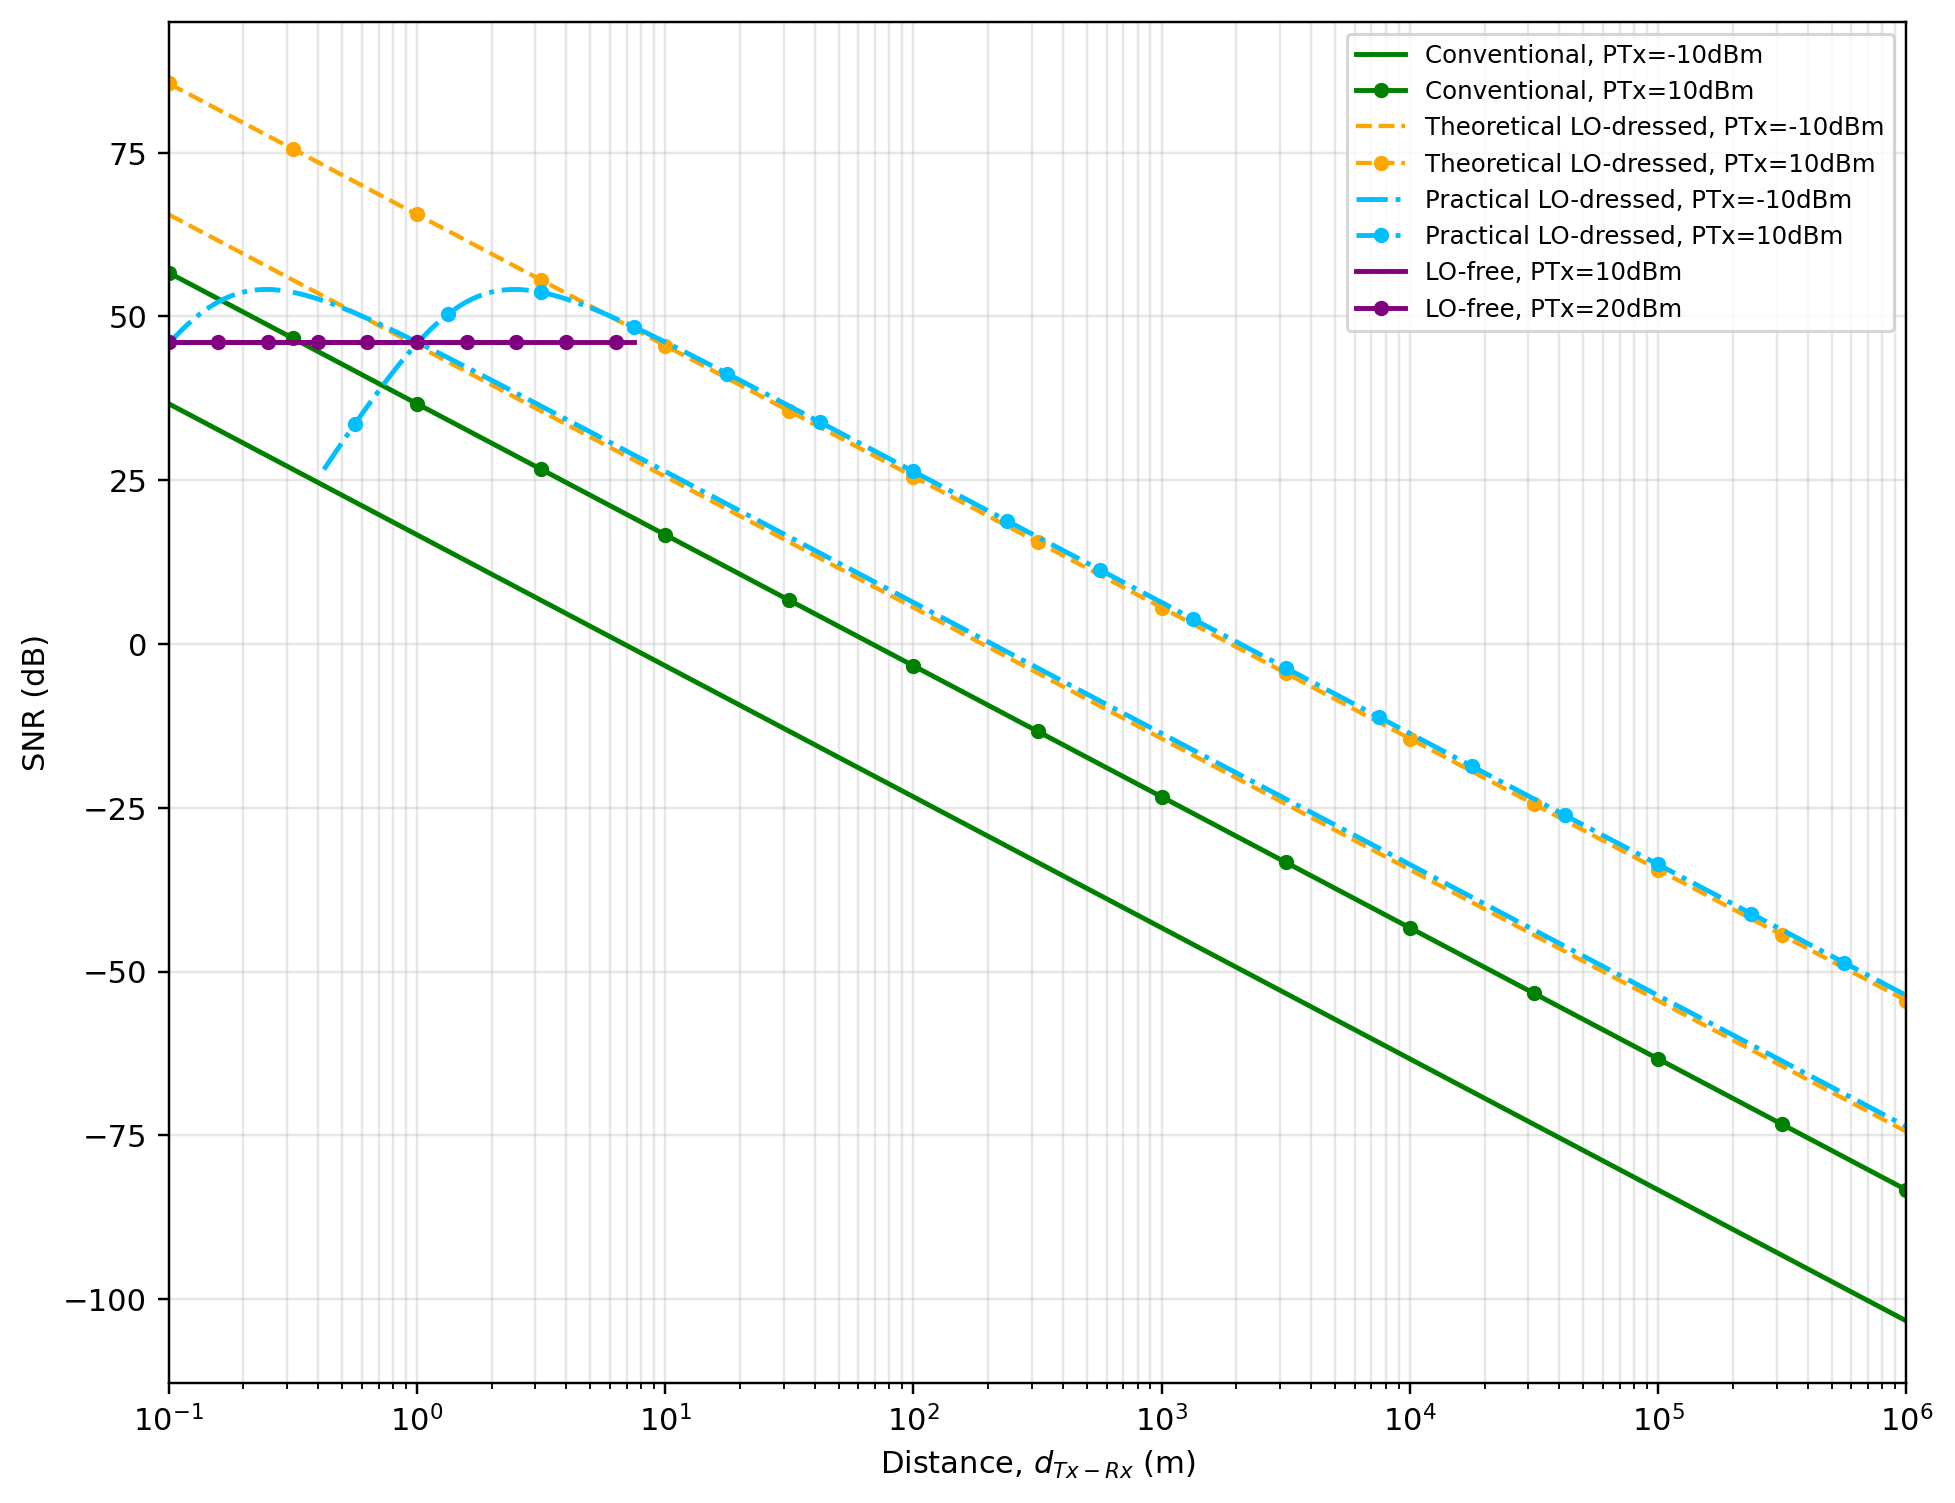
\includegraphics[width=\linewidth,height=0.72\textheight,keepaspectratio]{h_fig6_snr_distance.png}\\
  {\tiny SNR versus distance (Fig.~6 of~\cite{chen2025harnessing})}
\end{center}
\column{0.45\textwidth}
\footnotesize
\textbf{Graph generation}
\begin{itemize}\setlength\itemsep{1pt}
  \item $d\to P_{Rx}=P_{Tx}G_{Tx}\eta_0/(4\pi d^2)\to\Omega_{RF}\propto\sqrt{P_{Rx}}$
  \item LO-free: plotted only where $\Omega_{RF}\geq\Omega_{RF,th}$
  \item Practical LO-dressed: $\Omega_{total}(t)\to P_{out}(t)\to|P(\Delta f)|\to$ SNR
\end{itemize}
\vspace{1mm}
\textbf{Observations}
\begin{itemize}\setlength\itemsep{1pt}
  \item LO-free SNR saturates at $1/\tilde\epsilon^2=46.02$~dB
  \item Practical LO-dressed is worse at short range (outside linear range)
  \item LO-dressed gain at 100~m: 28.9~dB (paper $\approx44$~dB)
\end{itemize}
\end{columns}
\end{frame}

%% =========================================================
%% PART B: Xu et al.
%% =========================================================

%% ---- 11. Atomic MIMO model -------------------------------
\begin{frame}{Part B~\cite{xu2025channel}: Atomic MIMO Model and Linearisation}
\vspace*{-4mm}
\begin{columns}[T]
\column{0.50\textwidth}
\footnotesize
\setlength{\abovedisplayskip}{3pt}\setlength{\belowdisplayskip}{3pt}
\textbf{Measurement at cell $i$, pilot slot $p$}~\cite{cui2025towards,xu2025channel}
\[
  y_{i,p}=\Big|\sum_{k=1}^K g_{i,k}s_{k,p}+b_{i,p}+n_{i,p}\Big|
\]
\textbf{User channel} ($L_k$ paths)
\[
  g_{i,k}=\sum_{l=1}^{L_k}\frac{1}{\hbar}\bm\mu_{eg}^T\bm\epsilon_{i,k,l}\,\alpha_{l,k}\,e^{-j(i-1)\varphi_{l,k}}
\]
\textbf{Reference signal} (known, from a nearby source)
\[
  b_{i,p}=\frac{s_{b,p}}{\hbar}\,\alpha_b\,\bm\mu_{eg}^T\bm\epsilon_{b,i}\,e^{-j(i-1)\varphi_b}
\]
\begin{itemize}\setlength\itemsep{1pt}
  \item $n_{i,p}\sim\mathcal{CN}(0,\sigma^2)$; $\bm\epsilon$: polarisation; $\alpha$: path gain
  \item Only the magnitude is measured, so LS/MMSE cannot be used directly
\end{itemize}
\column{0.47\textwidth}
\footnotesize
\setlength{\abovedisplayskip}{3pt}\setlength{\belowdisplayskip}{3pt}
\textbf{First-order linearisation} (if $|b|\gg|a+n|$, $a_{i,p}=\sum_kg_{i,k}s_{k,p}$)
\[
  y_{i,p}\approx|b_{i,p}|+\mathrm{Re}\{e^{-j\angle b_{i,p}}a_{i,p}\}+\bar n_{i,p}
\]
{\scriptsize with $\bar n_{i,p}=\mathrm{Re}\{e^{-j\angle b_{i,p}}n_{i,p}\}\sim\mathcal N(0,\sigma^2/2)$}
\[
  \Longrightarrow\;\mathbf Y=\mathrm{Re}\{\mathbf Z\circ(\mathbf G\mathbf S)\}+|\mathbf B|+\mathbf N,\quad Z_{i,p}=e^{-j\angle b_{i,p}}
\]
\vspace{1mm}
\textbf{Strong-reference condition}
\begin{itemize}\setlength\itemsep{3pt}
  \item Dropped term $\sim|a+n|^2/(2|b|)$: accuracy depends on the reference-to-signal ratio
  \item With the paper's parameters, $\mathbb E|b|^2/\mathbb E|a+n|^2\approx-2$~dB: the reference is weaker than the signal
  \item The linear model is then not valid and the NMSE of all estimators stalls near 0~dB
  \item Since the derivation assumes $|b|\gg|a+n|$, the reference is scaled to $\mathbb E|b|^2/\mathbb E|a|^2=34$~dB and kept fixed over the pilot slots, as in~\cite{cui2025towards}
\end{itemize}
\end{columns}
\end{frame}

%% ---- 12. GD + GS -----------------------------------------
\begin{frame}{Part B~\cite{xu2025channel}: GD and Biased GS Algorithms (1D Array)}
\begin{columns}[T]
\column{0.49\textwidth}
\centering
\small\textbf{Gradient descent (GD)}~\cite{xu2025channel}\\[1pt]
{\scriptsize Cost $\mathcal L(\mathbf G)=\big\|\mathbf Y-|\mathbf B|-\mathrm{Re}\{\mathbf Z\circ(\mathbf G\mathbf S)\}\big\|_F^2$ (linearised model)}\\[3pt]
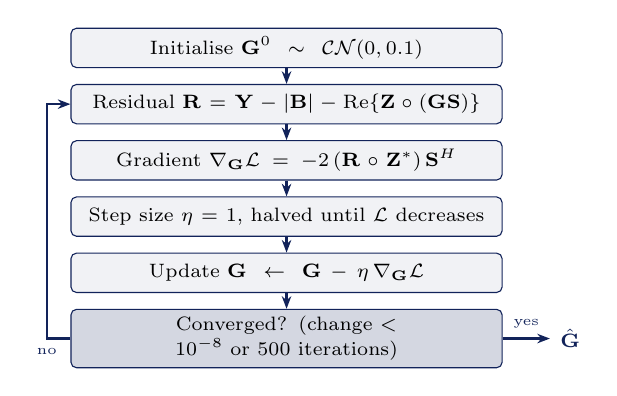
\begin{tikzpicture}[node distance=2mm]
  \node[fc] (a1) {Initialise $\mathbf G^0\sim\mathcal{CN}(0,0.1)$};
  \node[fc, below=of a1] (a2) {Residual $\mathbf R=\mathbf Y-|\mathbf B|-\mathrm{Re}\{\mathbf Z\circ(\mathbf G\mathbf S)\}$};
  \node[fc, below=of a2] (a3) {Gradient $\nabla_{\mathbf G}\mathcal L=-2\,(\mathbf R\circ\mathbf Z^*)\,\mathbf S^H$};
  \node[fc, below=of a3] (a4) {Step size $\eta=1$, halved until $\mathcal L$ decreases};
  \node[fc, below=of a4] (a5) {Update $\mathbf G\leftarrow\mathbf G-\eta\,\nabla_{\mathbf G}\mathcal L$};
  \node[fcd, below=of a5] (a6) {Converged? (change $<10^{-8}$ or 500 iterations)};
  \draw[fa] (a1)--(a2); \draw[fa] (a2)--(a3); \draw[fa] (a3)--(a4);
  \draw[fa] (a4)--(a5); \draw[fa] (a5)--(a6);
  \draw[fa] (a6.west) -- ++(-3mm,0) node[below,font=\tiny]{no} |- (a2.west);
  \draw[fa] (a6.east) -- node[above,font=\tiny]{yes} ++(6mm,0) node[right,font=\scriptsize]{$\hat{\mathbf G}$};
\end{tikzpicture}
\column{0.49\textwidth}
\centering
\small\textbf{Biased Gerchberg--Saxton (GS)}~\cite{cui2025towards}\\[1pt]
{\scriptsize Run for each cell $i$ on the exact magnitude model}\\[3pt]
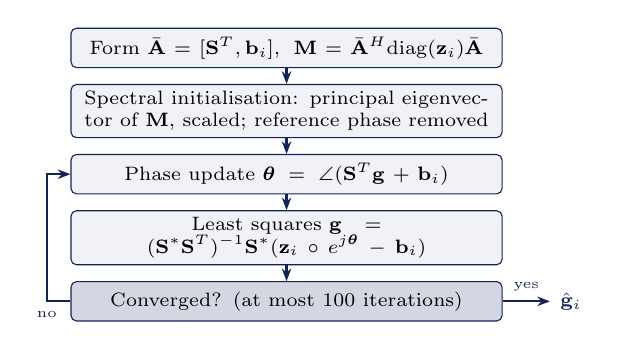
\begin{tikzpicture}[node distance=2mm]
  \node[fc] (b1) {Form $\bar{\mathbf A}=[\mathbf S^T,\mathbf b_i]$,\; $\mathbf M=\bar{\mathbf A}^H\mathrm{diag}(\mathbf z_i)\bar{\mathbf A}$};
  \node[fc, below=of b1] (b2) {Spectral initialisation: principal eigenvector of $\mathbf M$, scaled; reference phase removed};
  \node[fc, below=of b2] (b3) {Phase update $\bm\theta=\angle(\mathbf S^T\mathbf g+\mathbf b_i)$};
  \node[fc, below=of b3] (b4) {Least squares $\mathbf g=(\mathbf S^*\mathbf S^T)^{-1}\mathbf S^*(\mathbf z_i\circ e^{j\bm\theta}-\mathbf b_i)$};
  \node[fcd, below=of b4] (b5) {Converged? (at most 100 iterations)};
  \draw[fa] (b1)--(b2); \draw[fa] (b2)--(b3); \draw[fa] (b3)--(b4); \draw[fa] (b4)--(b5);
  \draw[fa] (b5.west) -- ++(-3mm,0) node[below,font=\tiny]{no} |- (b3.west);
  \draw[fa] (b5.east) -- node[above,font=\tiny]{yes} ++(6mm,0) node[right,font=\scriptsize]{$\hat{\mathbf g}_i$};
\end{tikzpicture}
\end{columns}
\vspace{2mm}
\begin{columns}[T]
\column{0.49\textwidth}\centering\scriptsize Uses the linearised model, so it inherits the Taylor error
\column{0.49\textwidth}\centering\scriptsize Exact model, but 1D only and no rank structure
\end{columns}
\end{frame}

%% ---- 13. PGD + CRLB --------------------------------------
\begin{frame}{Part B~\cite{xu2025channel}: PGD Algorithm (2D Array) and CRLB}
\begin{columns}[T]
\column{0.49\textwidth}
\centering
\small\textbf{Projected gradient descent (PGD)}~\cite{xu2025channel}\\[1pt]
{\scriptsize Mode-3 unfolding $\mathbf G_{(3)}\in\mathbb C^{K\times I_1I_2}$ of the channel tensor}\\[3pt]
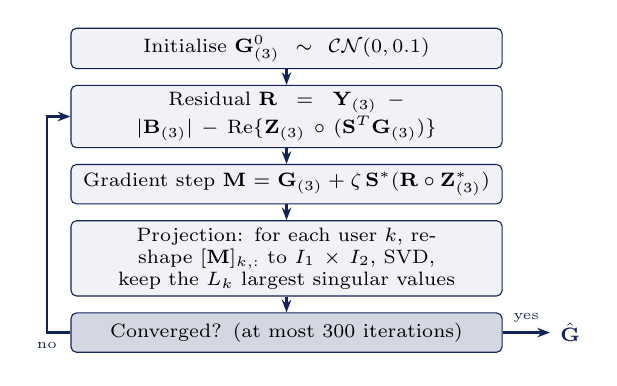
\begin{tikzpicture}[node distance=2mm]
  \node[fc] (c1) {Initialise $\mathbf G_{(3)}^0\sim\mathcal{CN}(0,0.1)$};
  \node[fc, below=of c1] (c2) {Residual $\mathbf R=\mathbf Y_{(3)}-|\mathbf B_{(3)}|-\mathrm{Re}\{\mathbf Z_{(3)}\circ(\mathbf S^T\mathbf G_{(3)})\}$};
  \node[fc, below=of c2] (c3) {Gradient step $\mathbf M=\mathbf G_{(3)}+\zeta\,\mathbf S^*(\mathbf R\circ\mathbf Z^*_{(3)})$};
  \node[fc, below=of c3] (c4) {Projection: for each user $k$, reshape $[\mathbf M]_{k,:}$ to $I_1\times I_2$, SVD, keep the $L_k$ largest singular values};
  \node[fcd, below=of c4] (c5) {Converged? (at most 300 iterations)};
  \draw[fa] (c1)--(c2); \draw[fa] (c2)--(c3); \draw[fa] (c3)--(c4); \draw[fa] (c4)--(c5);
  \draw[fa] (c5.west) -- ++(-3mm,0) node[below,font=\tiny]{no} |- (c2.west);
  \draw[fa] (c5.east) -- node[above,font=\tiny]{yes} ++(6mm,0) node[right,font=\scriptsize]{$\hat{\mathbf G}$};
\end{tikzpicture}\\[3pt]
{\scriptsize Each path is a rank-one outer product $\Rightarrow$ rank $\leq L_k$;\\
truncated SVD is the best rank-$L_k$ approximation (Eckart--Young--Mirsky)}
\column{0.49\textwidth}
\small\textbf{CRLB derivation}~\cite{xu2025channel}\\[2pt]
\footnotesize
\setlength{\abovedisplayskip}{3pt}\setlength{\belowdisplayskip}{3pt}
\begin{itemize}\setlength\itemsep{3pt}
  \item Vectorised linear model, $\mathbf g=\mathrm{vec}(\mathbf G)$:\\[2pt]
        $\mathbf y=\mathrm{Re}\{\mathbf z\circ(\mathbf I\otimes\mathbf S^T)\mathbf g\}+|\mathbf b|+\mathbf n$
  \item Real Gaussian noise; since $|z_{i,p}|=1$, $\;\mathbf I\circ(\mathbf z^*\mathbf z^T)=\mathbf I$
  \item Fisher information:
\end{itemize}
\[
  \mathrm{FIM}(\mathbf g)=\tfrac{1}{4\sigma^2}(\mathbf I\otimes\mathbf S^T)^H(\mathbf I\otimes\mathbf S^T)
  =\tfrac{1}{4\sigma^2}\,\mathbf I\otimes(\mathbf S^*\mathbf S^T)
\]
\begin{itemize}
  \item Inverting the FIM:
\end{itemize}
\[
  \mathrm{CRB}(\mathbf g)=4\sigma^2\big[\mathbf I_{I_1I_2}\otimes(\mathbf S^*\mathbf S^T)^{-1}\big]
\]
\begin{itemize}\setlength\itemsep{1pt}
  \item Per-cell bound does not depend on the number of cells
  \item Decreases with SNR ($\propto\sigma^2$) and with pilot length
\end{itemize}
\end{columns}
\end{frame}

%% ---- 14. CE: 1D ------------------------------------------
\begin{frame}{Part B~\cite{xu2025channel}: 1D Array Results}
\begin{columns}[T]
\column{0.56\textwidth}
\begin{center}
  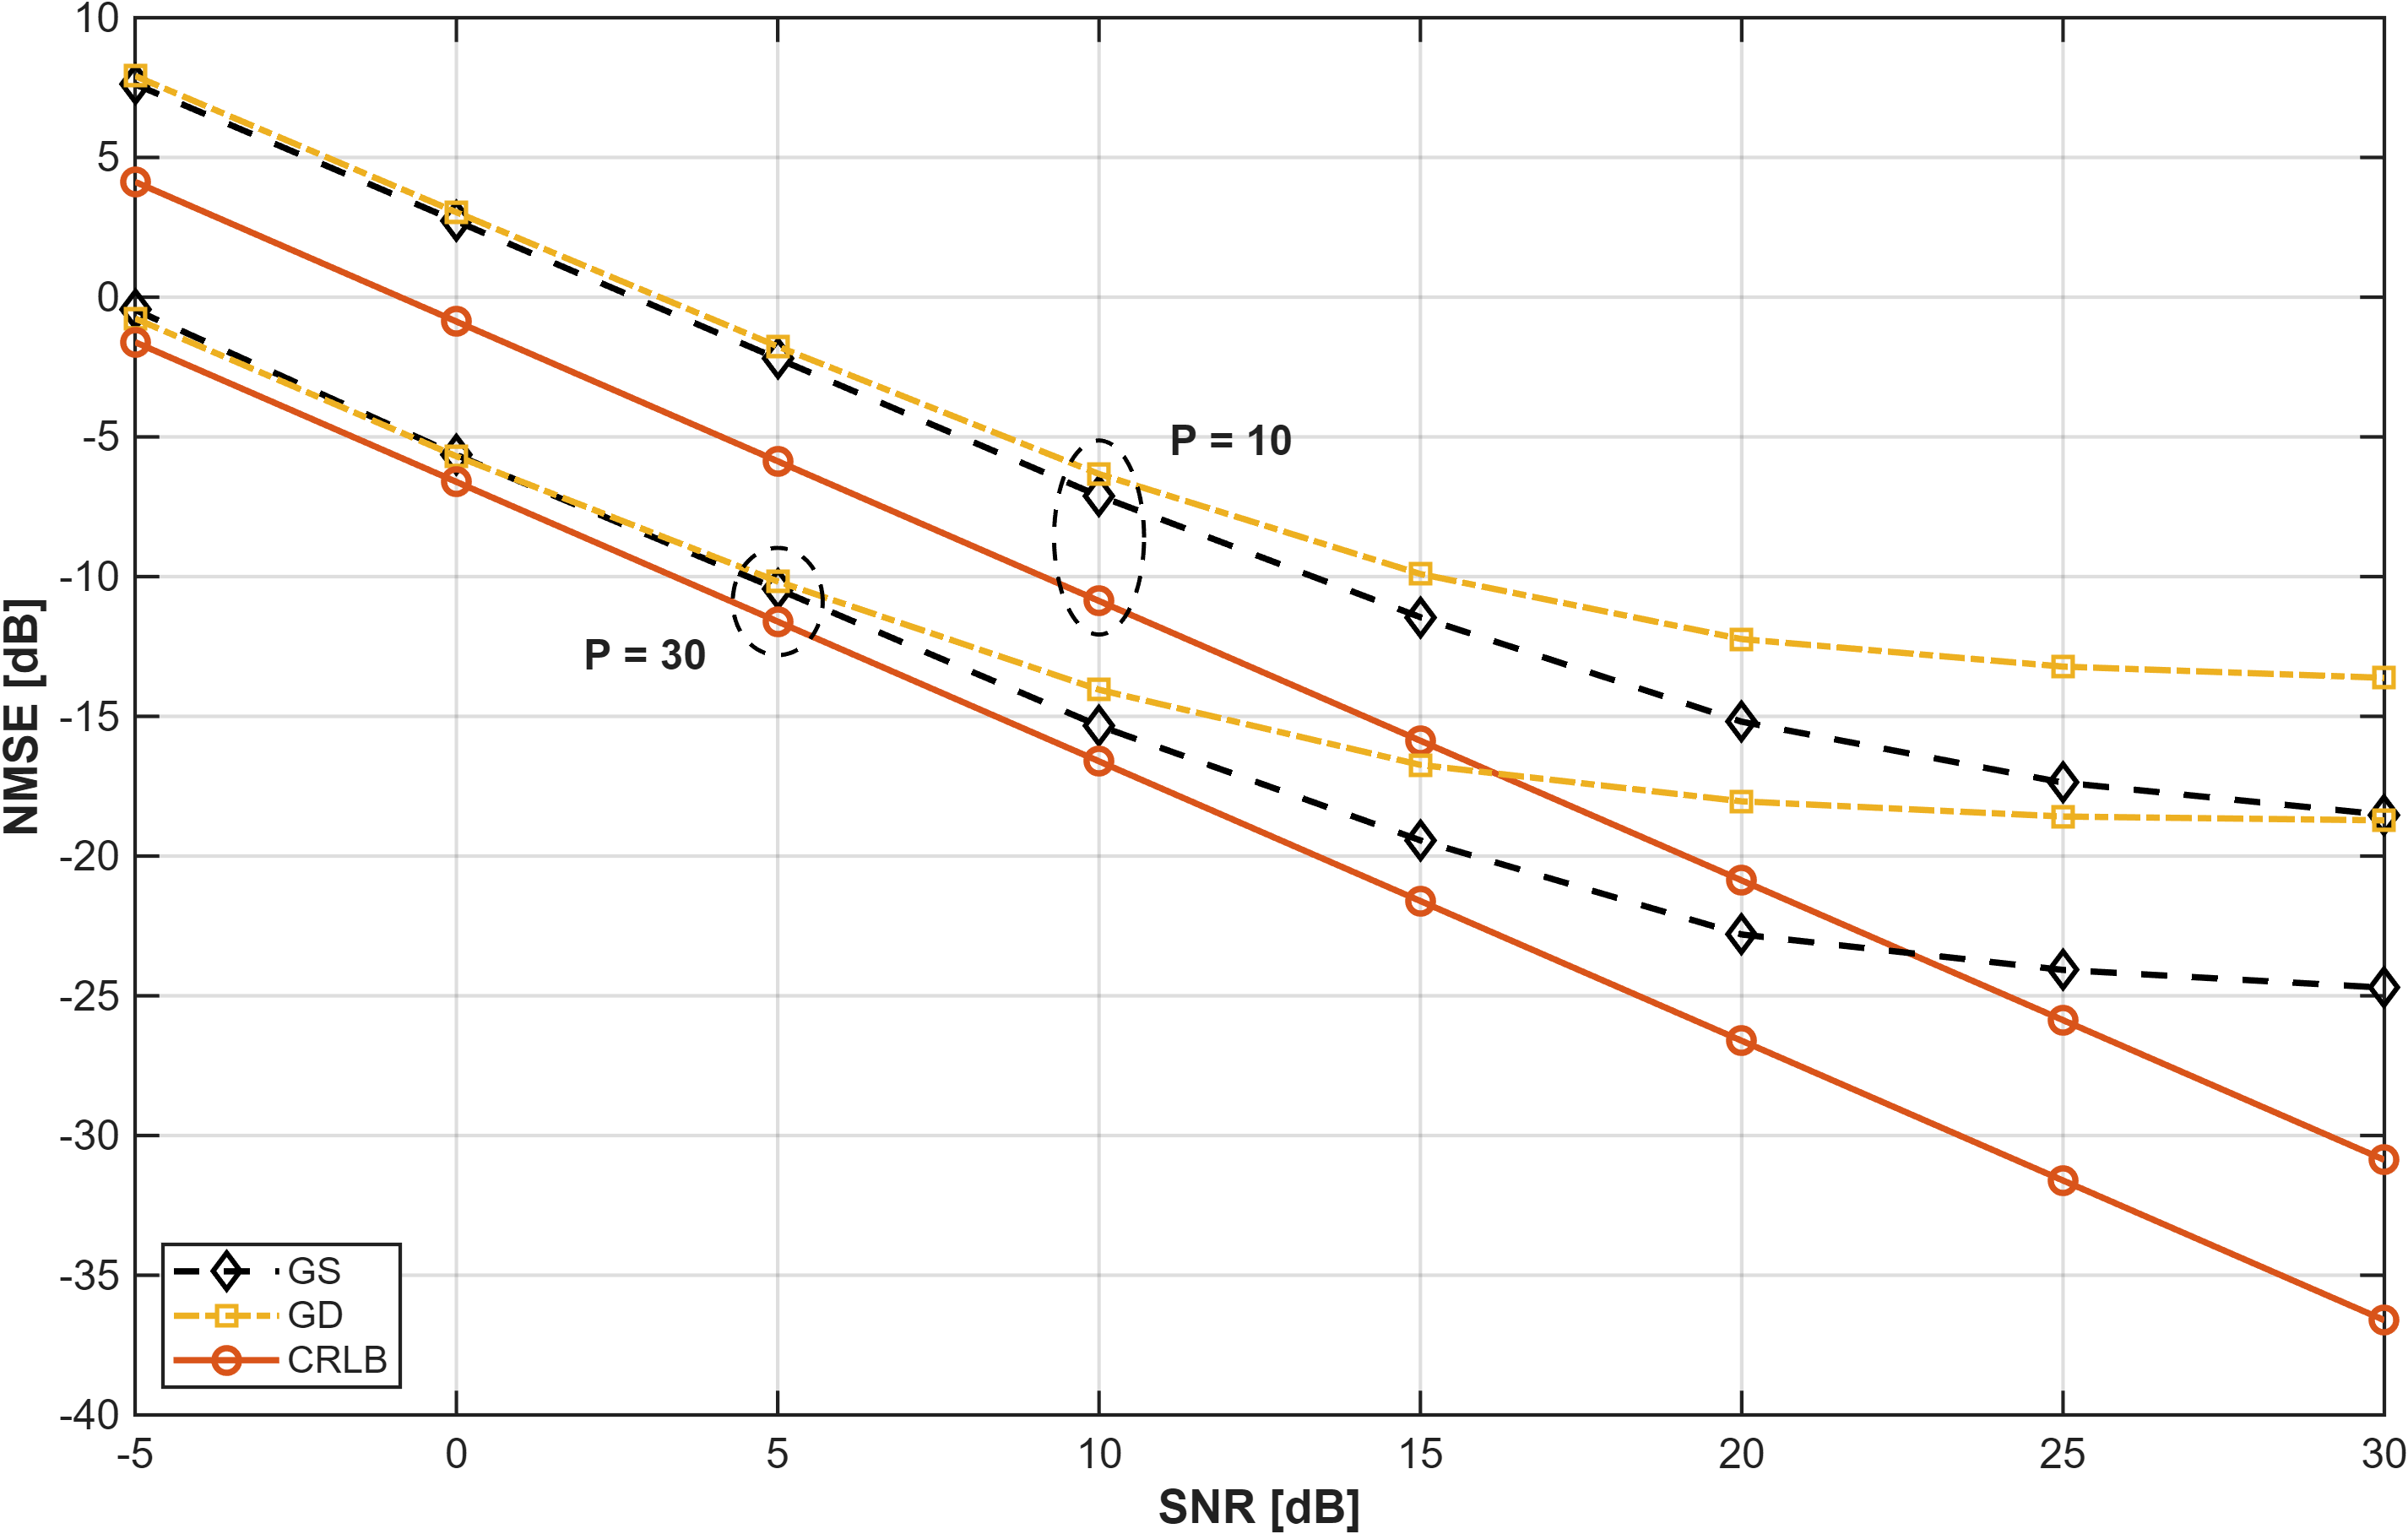
\includegraphics[width=\linewidth,height=0.70\textheight,keepaspectratio]{ce_fig3_1d.png}\\
  {\tiny NMSE vs SNR, 1D array ($I=8$, $K=3$): biased GS, GD, CRLB}
\end{center}
\column{0.41\textwidth}
\footnotesize
\textbf{Setup}
\begin{itemize}\setlength\itemsep{1pt}
  \item $K=3$, $L_k\in\{3,\dots,7\}$, $I=8$ (1D), $8\times8$ (2D)
  \item NMSE $=\sum\|\mathbf G-\hat{\mathbf G}\|_F^2/\sum\|\mathbf G\|_F^2$; 500 Monte Carlo runs
\end{itemize}
\vspace{1mm}
\textbf{Observations}
\begin{itemize}\setlength\itemsep{3pt}
  \item $P=30$: both close to the CRLB at low and medium SNR (at 5~dB: GS $-10.5$, GD $-10.2$, CRLB $-11.6$~dB)
  \item $P=10$: both about 4~dB above the bound
  \item GD flattens at high SNR ($\approx-18.7$~dB, $P=30$): the second-order Taylor term dominates once the noise is small
  \item GS uses the exact model and flattens lower ($-24.7$~dB), so curves for different $P$ can meet at high SNR
\end{itemize}
\end{columns}
\end{frame}

%% ---- 15. CE: 2D + pilots ---------------------------------
\begin{frame}{Part B~\cite{xu2025channel}: 2D Array and Pilot Length}
\begin{columns}[T]
\column{0.49\textwidth}
\begin{center}
  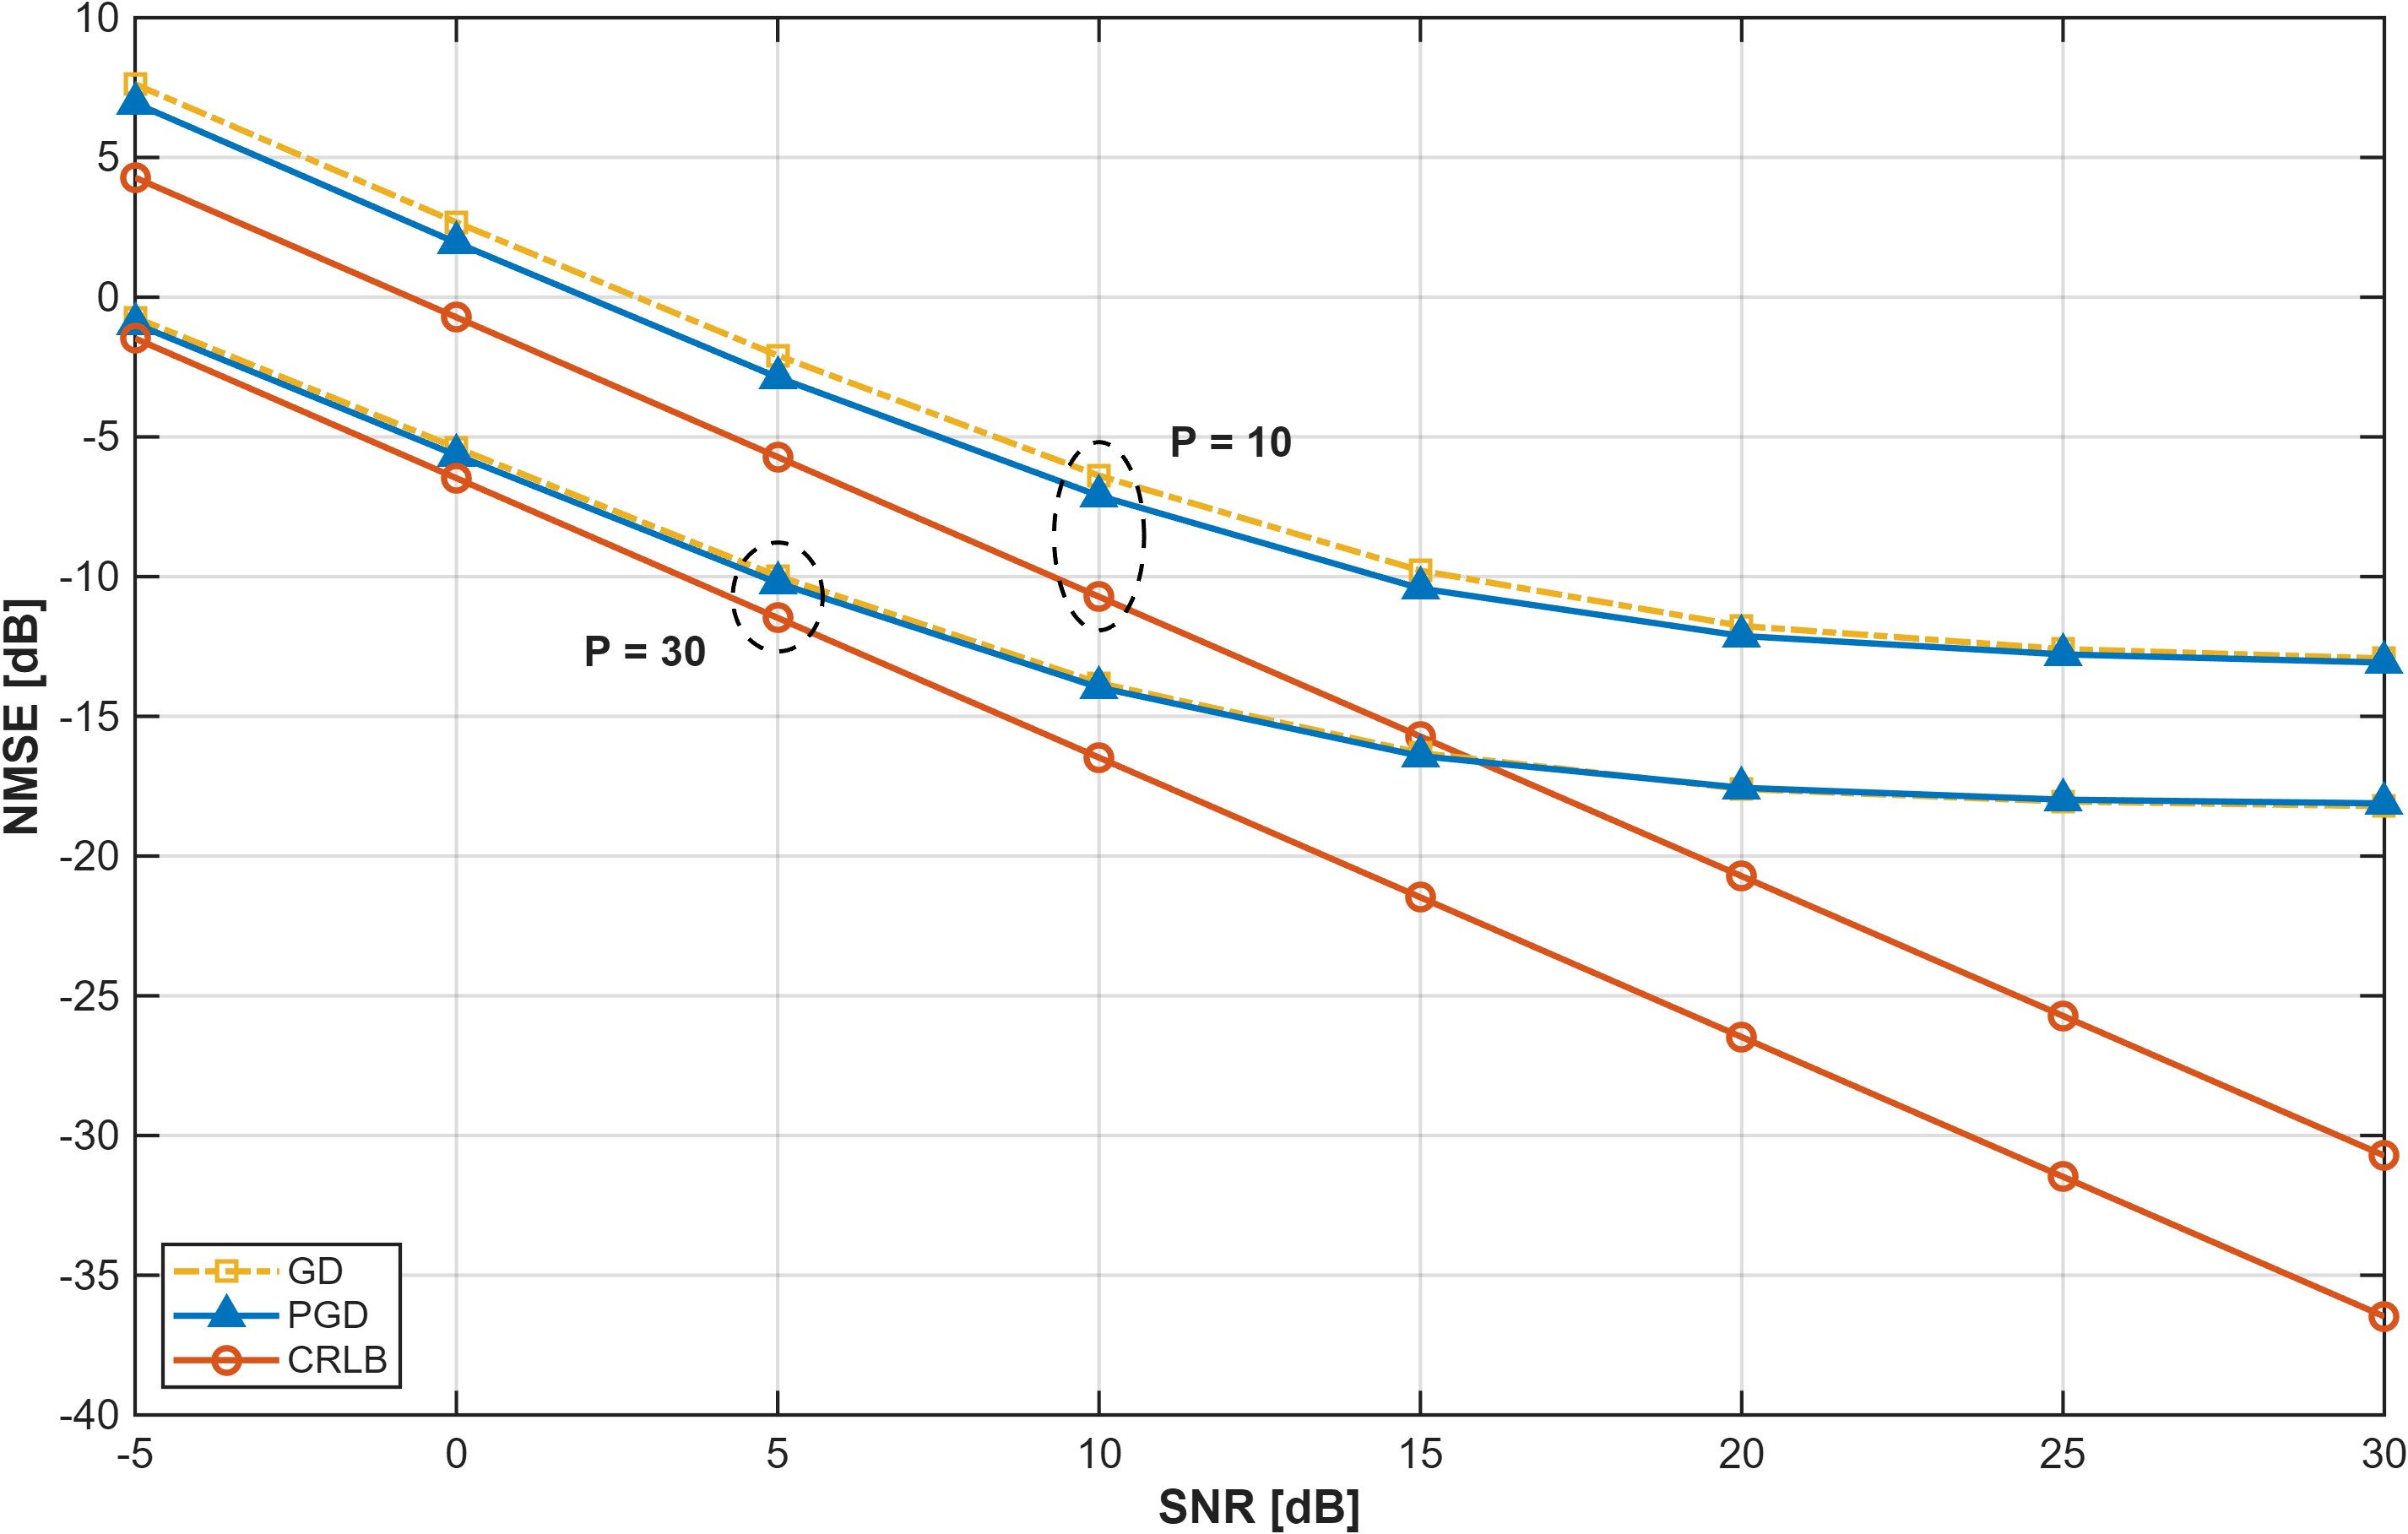
\includegraphics[width=\linewidth,height=0.52\textheight,keepaspectratio]{ce_fig4_2d.png}\\
  {\tiny NMSE vs SNR, $8\times8$ array: GD, PGD, CRLB}
\end{center}
\begin{itemize}\footnotesize\setlength\itemsep{1pt}
  \item $P=10$: PGD 0.6--0.8~dB better than GD (rank-$L_k$ projection)
  \item $P=30$: both within 1.3~dB of CRLB up to 5~dB SNR
\end{itemize}
\column{0.49\textwidth}
\begin{center}
  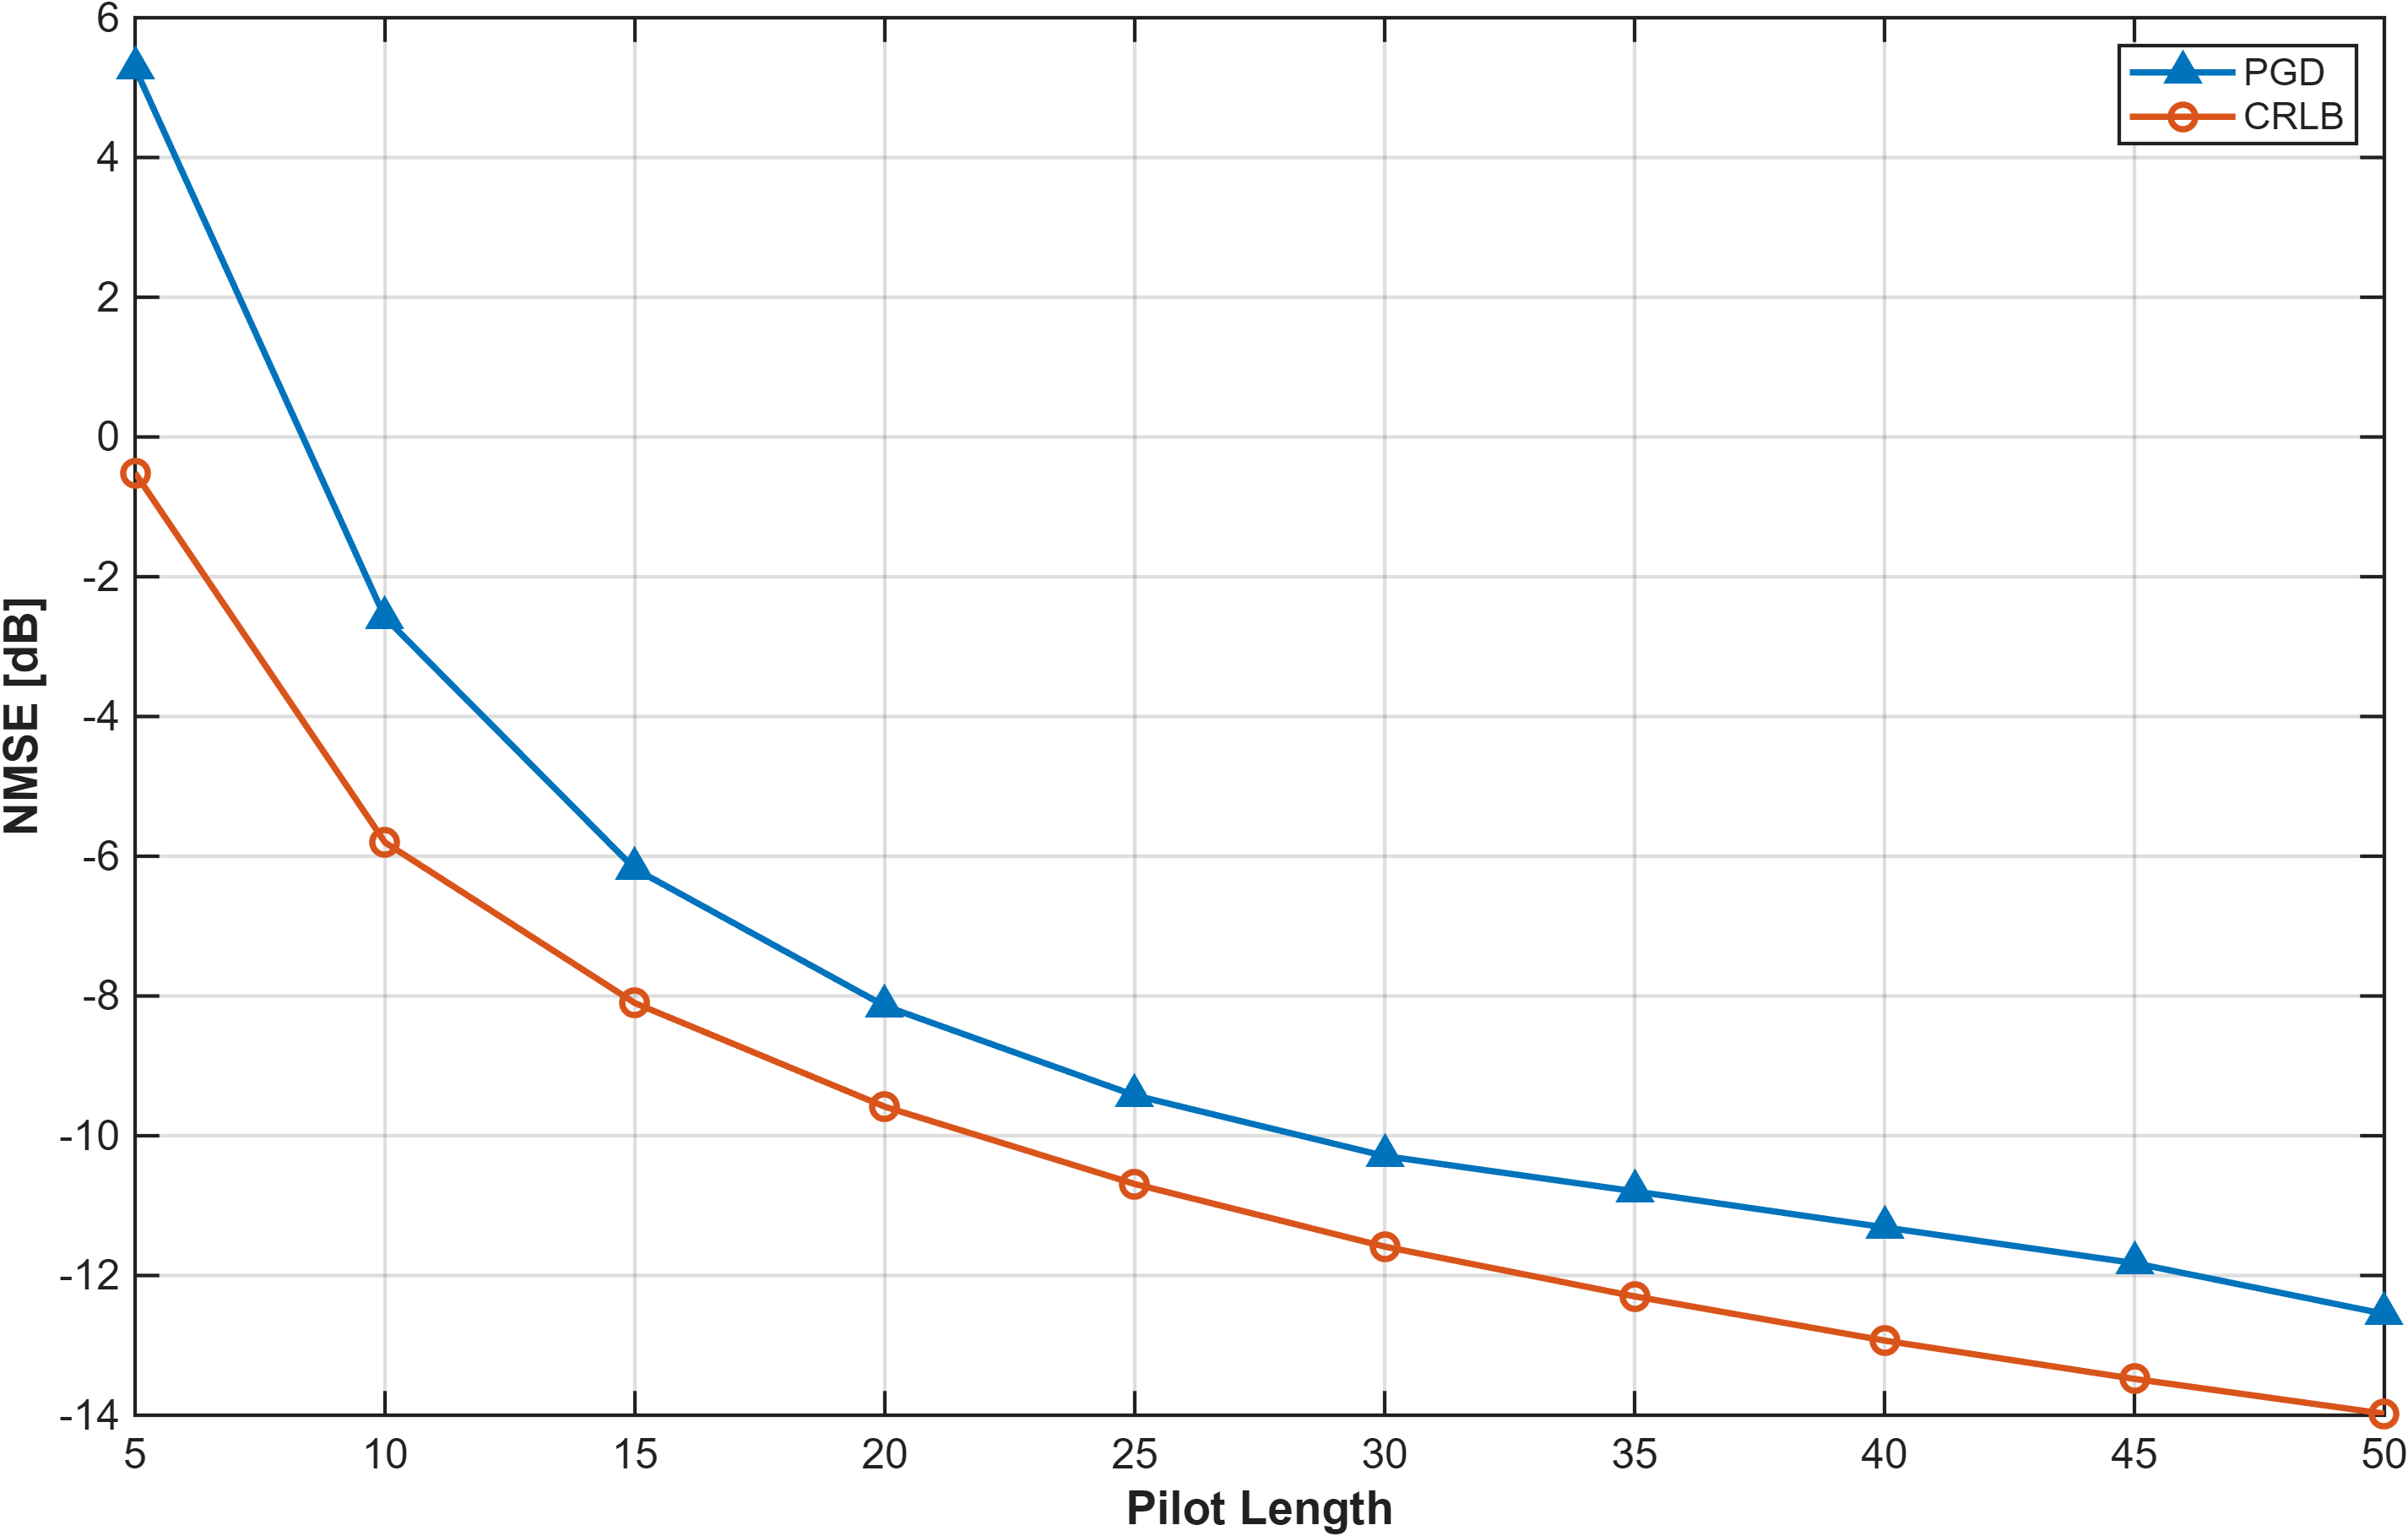
\includegraphics[width=\linewidth,height=0.52\textheight,keepaspectratio]{ce_fig5_pilot.png}\\
  {\tiny NMSE vs pilot length, $8\times8$ array, SNR = 5~dB}
\end{center}
\begin{itemize}\footnotesize\setlength\itemsep{1pt}
  \item Gap to CRLB: 5.8~dB ($P=5$) $\to$ 1.9~dB ($P=15$)
  \item 1.3--1.7~dB for $P\geq20$: about 20 pilots suffice
\end{itemize}
\end{columns}
\end{frame}

%% ---- 16. Gaps + future -----------------------------------
\begin{frame}{Research Gaps and Future Work}
\begin{columns}[T]
\column{0.49\textwidth}
\small\textbf{Research gaps}
\begin{enumerate}\footnotesize\setlength\itemsep{4pt}
  \item LO-dressed receiver analysed only for a single antenna~\cite{chen2025harnessing}
  \item LO-dressed and phase-retrieval models not compared or connected
  \item Estimators of~\cite{xu2025channel} rely on a strong reference; weak-reference case not studied
  \item Low-rank channel structure not used on the exact magnitude model
  \item Data-driven channel estimation not explored
\end{enumerate}
\column{0.49\textwidth}
\small\textbf{Future work}
\begin{enumerate}\footnotesize\setlength\itemsep{4pt}
  \item Study GS, EM-GS, GD and PGD across reference-to-signal ratios
  \item Channel estimator on the exact magnitude model using the rank structure, compared with the CRLB
  \item Channel estimation for arrays of LO-dressed receivers using the QuTiP response
  \item ML/DL-based channel estimation, suggested as an open problem in~\cite{cui2026rare}, compared with model-based estimators and the CRLB
\end{enumerate}
\end{columns}
\end{frame}

%% ---- 17. References --------------------------------------
\begin{frame}{References}
\scriptsize
\begin{thebibliography}{9}
\setbeamertemplate{bibliography item}{\insertbiblabel}

\bibitem{cui2026rare}
M.~Cui, Q.~Zeng, and K.~Huang, ``Rydberg atomic receiver: Next frontier of wireless
communications,'' \textit{arXiv:2412.12485v1}, Dec. 2024.

\bibitem{chen2025harnessing}
Y.~Chen \textit{et al.}, ``Harnessing Rydberg atomic receivers: From quantum physics to
wireless communications,'' \textit{arXiv:2501.11842v1}, Jan. 2025.

\bibitem{cui2025towards}
M.~Cui, Q.~Zeng, and K.~Huang, ``Towards atomic MIMO receivers,'' \textit{IEEE J. Sel.
Areas Commun.}, vol.~43, no.~3, pp.~659--673, Mar. 2025.

\bibitem{xu2025channel}
B.~Xu \textit{et al.}, ``Channel estimation for Rydberg atomic receivers,''
\textit{IEEE Wireless Commun. Lett.}, vol.~14, no.~9, pp.~2957--2961, Sep. 2025.

\bibitem{johansson2012qutip}
J.~R.~Johansson, P.~D.~Nation, and F.~Nori, ``QuTiP: An open-source Python framework for the
dynamics of open quantum systems,'' \textit{Comput. Phys. Commun.}, vol.~183, no.~8,
pp.~1760--1772, 2012.

\end{thebibliography}
\end{frame}

%% ---- Thank You -------------------------------------------
\begin{frame}[plain]
\begin{center}
  \vspace{1.5cm}
  {\Huge\textbf{Thank You}}\\[10pt]
  \rule{6cm}{0.5pt}
\end{center}
\end{frame}

\end{document}
